\chapter*{ECRICOME 2018 : le corrigé}
  
%

\section*{Exercice I}

\subsection*{Partie I}

\begin{noliste}{1.}
  \setlength{\itemsep}{4mm}
\item Soit $A$ la matrice de $\M{3}$ donnée par : $A =
  \begin{smatrix}
    2 & 1 & -2\\
    0 & 3 & 0\\
    1 & -1 & 5
  \end{smatrix}
  $.
  \begin{noliste}{a)}
    \setlength{\itemsep}{2mm}
  \item Calculer $A^{2}-7A$.

    \begin{proof}~%
      \begin{noliste}{$\sbullet$}
      \item Tout d'abord : $A^2 \ = \
        \begin{smatrix}
          2 & 1 & -2 \\
          0 & 3 & 0 \\
          1 & -1 & 5
        \end{smatrix}
        \begin{smatrix}
          2 & 1 & -2 \\
          0 & 3 & 0 \\
          1 & -1 & 5
        \end{smatrix}
        \ = \ 
        \begin{smatrix}
          2 & 7 & -14 \\
          0 & 9 & 0 \\
          7 & -7 & 23
        \end{smatrix}
        $.\\

      \item Ainsi : $A^2 - 7A =
        \begin{smatrix}
          2 & 7 & -14 \\
          0 & 9 & 0 \\
          7 & -7 & 23
        \end{smatrix}
        - 
        \begin{smatrix}
          14 & 7 & -14 \\
          0 & 21 & 0 \\
          7 & -7 & 35
        \end{smatrix}
        \ = \
        \begin{smatrix}
          -12 & 0 & 0 \\
          0 & -12 & 0 \\
          0 & 0 & -12
        \end{smatrix}
        \ = \ - 12 I_3$.
      \end{noliste}
      \conc{On en conclut : $A^2 - 7A = -12 I_3$.}~\\[-1.2cm]
    \end{proof}

  \item En déduire que les seuls réels susceptibles d'être valeurs
    propres de $A$ sont les réels $3$ et $4$.

    \begin{proof}~\\%
      D'après la question précédente, le polynôme $P(X) = X^2 - 7X +
      12 = (X-3)(X-4)$ est un polynôme annulateur de la matrice
      $A$.\\
      Or, le spectre de $A$ est inclus dans l'ensemble des racines
      d'un polynôme annulateur de $A$.%
      \conc{Ainsi, $\spc(A) \subset \{3, 4\}$. Les seuls réels
        susceptibles d'être valeurs propres de $A$ sont $3$ et
        $4$.}%~\\[-1.2cm]
      \begin{remark}~%
        \begin{noliste}{$\sbullet$}
        \item Une matrice $A \in \M{n}$ possède {\tt TOUJOURS} un
          polynôme annulateur non nul $P$.\\
          On peut même démontrer (ce n'est pas au programme en ECE)
          qu'il existe toujours un tel polynôme de degré (au plus)
          $n$.
          
        \item Si $P$ est un polynôme annulateur de $A$ alors, pour
          tout $\alpha \in \R$, le polynôme $\alpha \, P$ est toujours
          un polynôme annulateur puisque :
          \[
          (\alpha \, P)(A) = \alpha \, P(A) = 0
          \]
          Cela suffit à démontrer que $A$ possède une infinité de
          polynômes annulateurs. \\
          On peut en obtenir d'autres. Par exemple $Q(X) = (X-5) \
          P(X)$ est un polynôme annulateur de $A$ puisque :
          \[
          Q(A) = (A - 5 \, I) \ P(A) = 0
          \]
          Il faut donc parler {\tt D'UN} polynôme annulateur d'une
          matrice.
          
        \item Les racines d'un polynôme annulateur ne sont pas forcément
          toutes valeurs propres de $A$. Si c'était le cas, $A$ aurait
          une infinité de valeurs propres (elle en possède au plus $3$
          !). Par exemple, comme $Q(X) = (X-5) \ P(X)$ est un polynôme
          annulateur, un tel raisonnement permettrait de démontrer que
          $5$ est aussi valeur propre.
          
%         \item On dit généralement que les racines d'un polynôme
%           annulateur sont des valeurs propres {\bf possibles} de $A$
%           (comprendre qu'elles sont potentiellement des valeurs
%           propres). Il faut alors démontrer qu'elles sont réellement des
%           valeurs propres.
        \end{noliste}
      \end{remark}~\\[-1.4cm]
    \end{proof}


    \newpage


  \item Trouver alors toutes les valeurs propres de $A$, et pour
    chacune d'entre elles, donner une base du sous-espace propre
    associé.

    \begin{proof}~%
      \begin{noliste}{$\sbullet$}
      \item Déterminons $E_3(A) = \{X \in \M{3,1} \ | \ (A - 3 \cdot
        I_3) \ X = 0_{\M{3,1}} \}$.\\
        Soit $X=
        \begin{smatrix}
          x\\
          y\\
          z
        \end{smatrix}\in \M{3,1}$.
        \[
        \begin{array}{rcl}
          X\in E_3(A) & \Longleftrightarrow & (A-3 \cdot I_3) \ X = 0_{\M{3,1}}
          \\[.2cm]
          & \Longleftrightarrow & 
          \begin{smatrix}
            -1 & 1 & -2\\
            0 & 0 & 0\\
            1 & -1 & 2
          \end{smatrix}
          \begin{smatrix}
            x\\
            y\\
            z
          \end{smatrix}
          =
          \begin{smatrix}
            0\\
            0\\
            0
          \end{smatrix}
          \\[.8cm]
          & \Longleftrightarrow &
          \left\{
            \begin{array}{rcrcrcl}
              -x & + & y & - & 2z & = & 0\\
              & & & & 0 & = & 0\\
              x & - & y & + & 2z & = & 0
            \end{array}
          \right.
          \\[.8cm]
          &
          \begin{arrayEq}
            L_3 \leftarrow L_3 + L_1
          \end{arrayEq}
          &
          \left\{
            \begin{array}{rcrcrcl}
              -x & + & y & - & 2z & = & 0\\
              & & & & 0 & = & 0\\
              & & & & 0 & = & 0
            \end{array}
          \right.
          \\[.8cm]
          &
          \Longleftrightarrow
          &
          \left\{
            \begin{array}{rcrcrcl}
              -x & + & y & - & 2z & = & 0\\
            \end{array}
          \right.
        \end{array}
        \]
        Finalement, on obtient l'expression de $E_3(A)$ suivante :
        \[
        \begin{array}{rcl}
          E_3(A) & = & \{
          \begin{smatrix}
            x\\
            y\\
            z
          \end{smatrix}
          \in \M{3,1} \ | \ x = y - 2z \}
          \\[.6cm]
          & = & \{
          \begin{smatrix}
            y - 2z \\
            y \\
            z
          \end{smatrix}
          \ | \ (y, z) \in \R^2 \}
          \\[.6cm]
          & = & %
          \{ y \cdot
          \begin{smatrix}
            1 \\
            1 \\
            0
          \end{smatrix}
          +
          z \cdot
          \begin{smatrix}
            - 2 \\
            0 \\
            1
          \end{smatrix}
          \ | \ (y, z) \in \R^2 \}
          %\\[.8cm]
          \ = \ \Vect{
            \begin{smatrix}
              1 \\
              1 \\
              0
            \end{smatrix}
            ,
            \begin{smatrix}
              -2 \\
              0 \\
              1
            \end{smatrix}
          }
        \end{array}
        \]   
        Comme $E_3(A) \neq \{0_{\M{3,1}}\}$, $3$ est bien valeur
        propre de $A$, d'espace propre associé $E_3(A)$.%
        \conc{$E_3(A) \ = \ \Vect{
            \begin{smatrix}
              1 \\
              1 \\
              0
            \end{smatrix}
            ,
            \begin{smatrix}
              -2 \\
              0 \\
              1
            \end{smatrix}
          }$}
        \begin{remarkL}{.97}%~
          Il est important de lire l'énoncé de ce type de questions en
          entier pour choisir une méthode de résolution. En effet :
          \begin{noliste}{$\stimes$}
          \item si l'énoncé demande simplement de montrer qu'un réel
            $\lambda$ donné est valeur propre d'une matrice $A$ carrée
            d'ordre $3$, alors on vérifie $\rg(A-\lambda \, I_3) < 3$
            pour ce réel $\lambda$ particulier.\\
            {\it (si $A$ est une matrice carrée d'ordre $2$, on
              vérifie $\det(A-\lambda \, I_2)=0_{\R}$)}
          \item si l'énoncé demande de montrer qu'un réel $\lambda$
            est valeur propre d'une matrice $A$ carrée d'ordre $3$
            {\bf et} de déterminer le sous-espace propre associé,
            alors on détermine directement $E_\lambda(A)$ et comme
            $E_\lambda(A) \neq \{0_{\M{3,1}}\}$, cela démontre que
            $E_\lambda(A)$ est bien le sous-espace propre associé à la
            valeur propre $\lambda$.
          \end{noliste}
        \end{remarkL}


        \newpage


      \item Déterminons $E_4(A) = \{X \in \M{3,1} \ | \ (A - 4 \cdot
        I_3) \ X = 0_{\M{3,1}} \}$.\\
        Soit $X=
        \begin{smatrix}
          x\\
          y\\
          z
        \end{smatrix} \in \M{3,1}$.
        \[
        \begin{array}{rcl}
          X \in E_4(A) & \Longleftrightarrow & (A-4 \cdot I_3) \ X =
          0_{\M{3,1}} 
          \\[.2cm]
          & \Longleftrightarrow & 
          \begin{smatrix}
            -2 & 1 & -2\\
            0 & -1 & 0\\
            1 & -1 & 1
          \end{smatrix}
          \begin{smatrix}
            x\\
            y\\
            z
          \end{smatrix}
          =
          \begin{smatrix}
            0\\
            0\\
            0
          \end{smatrix}
          \\[.8cm]
          & \Longleftrightarrow &
          \left\{
            \begin{array}{rcrcrcl}
              -2x & + & y & - & 2z & = & 0\\
              & - & y & & 0 & = & 0\\
              x & - & y & + & z & = & 0
            \end{array}
          \right.
          \\[.8cm]
          &
          \begin{arrayEq}
            L_3 \leftarrow 2 \ L_3 + L_1
          \end{arrayEq}
          &
          \left\{
            \begin{array}{rcrcrcl}
              -2x & + & y & - & 2z & = & 0\\
              & - & y & & & = & 0\\
              & - & y & & & = & 0
            \end{array}
          \right.
          \\[.8cm]
          &
          \Longleftrightarrow
          &
          \left\{
            \begin{array}{rcrcr}
              -2x & + & y & = & 2z \\
              & - & y & = & 0 
            \end{array}
          \right.
          \\[.8cm]
          &
          \begin{arrayEq}
            L_1 \leftarrow L_1 + L_2
          \end{arrayEq}
          &
          \left\{
            \begin{array}{rcrcr}
              -2x & & & = & 2z \\
              & - & y & = & 0 
            \end{array}
          \right.
        \end{array}
        \]
        Finalement, on obtient l'expression de $E_4(A)$ suivante :
        \[
        \begin{array}{rcl}
          E_4(A) & = & \{
          \begin{smatrix}
            x\\
            y\\
            z
          \end{smatrix}
          \in \M{3,1} \ | \ x = -z \ \text{ et } \ y = 0 \}
          \\[.6cm]
          & = & \{
          \begin{smatrix}
            -z \\
            0 \\
            z
          \end{smatrix}
          \ | \ z \in \R \}
          %\\[.6cm]
          \ = \ %
          \{ z \cdot
          \begin{smatrix}
            -1 \\
            0 \\
            1
          \end{smatrix}
          \ | \ z \in \R \}
          % \\[.8cm]
          \ = \ \Vect{
            \begin{smatrix}
              -1 \\
              0 \\
              1
            \end{smatrix}
          }
        \end{array}
        \]   
        Comme $E_4(A) \neq \{0_{\M{3,1}}\}$, $4$ est bien valeur
        propre de $A$, d'espace propre associé $E_4(A)$.%
        \conc{$E_4(A) \ = \ \Vect{
            \begin{smatrix}
              -1 \\
              0 \\
              1
            \end{smatrix}
          }$}~\\[-1.4cm]
      \end{noliste}
    \end{proof}

  \item La matrice $A$ est-elle inversible ? Est-elle diagonalisable ?

    \begin{proof}~%
      \begin{noliste}{$\sbullet$}
      \item D'après la question précédente, $0$ n'est pas valeur
        propre de $A$.%
        \conc{Ainsi, $A$ est inversible.}

      \item Déterminons les dimensions des sous-espaces propres.\\
        La famille ${\cal F}_1 = \left(
          \begin{smatrix}
            1 \\
            1 \\
            0
            \end{smatrix}
            ,
            \begin{smatrix}
            -2 \\
            0 \\
            1
            \end{smatrix}
          \right)$ :
          \begin{noliste}{$\stimes$}
          \item engendre $E_3(A)$,
          \item est libre car constituée de deux vecteurs non
            colinéaires.
          \end{noliste}
          Ainsi, ${\cal F}_1$ est une base de $E_3(A)$.%
          \conc{On en déduit : $\dim\big( E_3(A) \big) = \Card\big(
            {\cal F}_1 \big) = 2$.}%


          \newpage


          \noindent
          La famille ${\cal F}_2 = \left(
          \begin{smatrix}
            -1 \\
            0 \\
            1
            \end{smatrix}
          \right)$ :
          \begin{noliste}{$\stimes$}
          \item engendre $E_4(A)$,
          \item est libre car constituée d'un vecteur non nul.
          \end{noliste}
          Ainsi, ${\cal F}_2$ est une base de $E_4(A)$.%
          \conc{On en déduit : $\dim\big( E_4(A) \big) = \Card\big(
            {\cal F}_2 \big) = 1$.}%

      \item La matrice $A$ est un matrice carrée d'ordre $3$. Or :
        \[
        \dim\big( E_3(A) \big) + \dim\big( E_4(A) \big) \ = \ 3
        \]
        \conc{On en déduit que $A$ est diagonalisable.}~\\[-1.2cm]
      \end{noliste}
    \end{proof}

  \end{noliste}

\item Soit $\B = (e_{1},e_{2},e_{3})$ la base canonique de $\R^{3}$ et
  $f$ l'endomorphisme de $\R^{3}$ dont la matrice représentative dans
  la base $\B$ est la matrice : $B =
  \begin{smatrix}
    1 & -1 & -1\\
    -3 & 3 & -3\\
    -1 & 1 & 1
  \end{smatrix}
  $.
  \begin{noliste}{a)}
    \setlength{\itemsep}{2mm}
  \item Déterminer le noyau de $f$. En déduire une valeur propre de
    $f$ et l'espace propre associé.

    \begin{proof}~%
      \begin{noliste}{$\sbullet$}
      \item Soit $u = (x, y, z) \in \R^3$ et notons $U = \Mat_{\B}(u)
        =
        \begin{smatrix}
          x\\
          y\\
          z
        \end{smatrix} \in \M{3,1}$.
        \[
        \begin{array}{rcl}
          u \in \kr(f) & \Longleftrightarrow & f(u) = 0_{\R^3} 
          \\[.2cm]
          & \Longleftrightarrow & B U = 0_{\M{3,1}} 
          \\[.2cm]
          & \Longleftrightarrow & 
          \begin{smatrix}
            1 & -1 & -1\\
            -3 & 3 & -3\\
            -1 & 1 & 1
          \end{smatrix}
          \begin{smatrix}
            x\\
            y\\
            z
          \end{smatrix}
          =
          \begin{smatrix}
            0\\
            0\\
            0
          \end{smatrix}
          \\[.8cm]
          & \Longleftrightarrow &
          \left\{
            \begin{array}{rcrcrcl}
              x & - & y & - & z & = & 0\\
              -3x & + & 3y & - & 3z & = & 0\\
              -x & + & y & + & z & = & 0
            \end{array}
          \right.
          \\[.8cm]
          &
          \begin{arrayEq}
            L_2 \leftarrow L_2 + 3 \ L_1 \\
            L_3 \leftarrow L_3 + L_1 
          \end{arrayEq}
          &
          \left\{
            \begin{array}{rcrcrcl}
              x & - & y & - & z & = & 0\\
              & & & - & 6z & = & 0\\
              & & & & 0 & = & 0
            \end{array}
          \right.
          \\[.8cm]
          &
          \Longleftrightarrow
          &
          \left\{
            \begin{array}{rcrcr}
              x & - & z & = & y \\
              & & z & = & 0 
            \end{array}
          \right.
          \\[.8cm]
          &
          \begin{arrayEq}
            L_1 \leftarrow L_1 + L_2
          \end{arrayEq}
          &
          \left\{
            \begin{array}{rcrcr}
              x & & & = & y \\
              & & z & = & 0 
            \end{array}
          \right.
        \end{array}
        \]
        Finalement, on obtient l'expression de $\kr(f)$ suivante :
        \[
        \begin{array}{rcl}
          \kr(f) & = & \{
          (x, y, z) \in \R^3 \ | \ x = y \ \text{ et } \ z = 0 \}
          \\[.2cm]
          & = & \{
          (y, y, 0) \ | \ y \in \R \}
          %\\[.6cm]
          \ = \ %
          \{ y \cdot
          (1, 1, 0) \ | \ y \in \R \}
          % \\[.8cm]
          \ = \ \Vect{
            (1, 1, 0)
          }
        \end{array}
        \]   
        \conc{$\kr(f) = \Vect{ (1, 1, 0) }$}


        \newpage


      \item Ainsi : $E_0(f) = \kr(f) = \Vect{ (1, 1, 0) } \neq \{
        0_{\R^3}\}$.%
        \conc{On en déduit que $0$ est valeur propre de $f$, d'espace
          propre associé $E_0(f) = \Vect{ (1, 1, 0) }$.}~\\[-1.2cm]        
      \end{noliste}
    \end{proof}

  \item Déterminer le rang de la matrice $B-2I_{3}$.

    \begin{proof}~%
      \[
      \begin{array}{rcl}
        \rg(B - 2I_3) & = & \rg %
        \left(
          \begin{smatrix}
            -1 & -1 & -1 \\
            -3 & 1 & -3 \\
            -1 & 1 & -1
          \end{smatrix}
          \right) %
          = %
          \rg %
          \left(
            \begin{smatrix}
              -1 \\ 
              -3 \\
              -1
            \end{smatrix}, %
            \begin{smatrix}
              - 1 \\ 
              1 \\
              1
            \end{smatrix}, %
            \begin{smatrix}
              -1 \\ 
              -3 \\
              -1
            \end{smatrix}          
          \right)
          \\[.8cm]
          & = &
          \dim( %
          \ \Vect{%
            \begin{smatrix}
              -1 \\ 
              -3 \\
              -1
            \end{smatrix}, %
            \begin{smatrix}
              - 1 \\ 
              1 \\
              1
            \end{smatrix}, %
            \begin{smatrix}
              -1 \\ 
              -3 \\
              -1
            \end{smatrix}          
          } \ ) %
          \\[.8cm]
          & = &
          \dim( \ %
          \Vect{%
            \begin{smatrix}
              -1 \\ 
              -3 \\
              -1
            \end{smatrix}, %
            \begin{smatrix}
              - 1 \\ 
              1 \\
              1
            \end{smatrix} %
          } \ ) %
          \ = \ 2
        \end{array}        
        \]
        En effet, la famille $\left( 
          \begin{smatrix}
            -1 \\
            -3 \\
            -1
          \end{smatrix}, %
          \begin{smatrix}
            - 1 \\ 
            1 \\
            1
          \end{smatrix}\right)$ est libre car constituée de deux
        vecteurs non colinéaires.%
        \conc{$\rg(B - 2 I_3) = 2$}~\\[-1cm]
    \end{proof}

  \item Calculer $f(e_{1} - e_{2} - e_{3})$.

    \begin{proof}~%
      \[
      \begin{array}{rcl}
        \Mat_{\B}\big( f(e_{1} - e_{2} - e_{3}) \big) & = &
        \Mat_{\B}(f) \times \Mat_{\B}(e_{1} - e_{2} - e_{3}) 
        \\[.2cm]
        & = & 
        \begin{smatrix}
          1 & -1 & -1\\
          -3 & 3 & -3\\
          -1 & 1 & 1
        \end{smatrix}
        \times 
        \begin{smatrix}
          1 \\
          -1 \\
          -1
        \end{smatrix}
        \ = \ 
        \begin{smatrix}
          3 \\
          -3 \\
          -3
        \end{smatrix}
        % \ = \ 3 \cdot 
        % \begin{smatrix}
        %   1 \\
        %   -1 \\
        %   -1
        % \end{smatrix}
      \end{array}
      \]
      \conc{On en déduit : $f(e_1 - e_2 - e_3) = (3, -3, -3)$.}~\\[-1.2cm]
    \end{proof}
    
  \item Déduire des questions précédentes que l'endomorphisme $f$ est
    diagonalisable.

    \begin{proof}~%
      \begin{noliste}{$\sbullet$}
      \item D'après la question \itbf{2.b)} : $\rg(B - 2I_3) = 2 <
        3$.\\
        On en déduit que la matrice $B - 2 I_3$ n'est pas
        inversible.\\
        Ainsi, $2$ est valeur propre de $B = \Mat_{\B}(f)$.%
        \conc{Le réel $2$ est valeur propre de $f$.}

      \item D'après la question \itbf{2.c)} :
        \[
        f(e_1 - e_2 - e_3) = (3, -3, -3) = 3 \cdot (1, -1, -1) = 3
        \cdot (e_1 - e_2 - e_3)
        \]
        \conc{Comme $e_1 - e_2 - e_3 \neq 0_{\R^3}$, le réel $3$ est
          valeur propre de $f$.}%~\\[-1.2cm]


        \newpage


      \item Enfin, on a démontré en \itbf{2.a)} que $0$ est valeur
        propre de $f$.\\
        L'application $f$ est un endomorphisme de $\R^3$ qui possède
        $3$ valeurs propres distinctes.%
        \conc{On en conclut que $f$ est diagonalisable.}
      \end{noliste}
        \begin{remark}%~
          \begin{noliste}{$\sbullet$}
          \item On peut aussi démontrer que $2$ est valeur propre de
            $f$ à l'aide du théorème du rang.\\
            Détaillons cette rédaction.
          \item Comme $B - 2I_3 = \Mat_{\B}(f - 2 \id)$, on en déduit
            : $\rg(f - 2 \id) = 2$.\\
            Ainsi, d'après le théorème du rang :
            \[
            \begin{array}{ccccc}
              \dim(\R^3) & = & \dim\big( \kr(f - 2 \id) \big) & + &
              \dim\big( \im (f - 2 \id) \big) 
              \\[.2cm]
              \shortparallel & & & & \shortparallel
              \\[.2cm]
              3 & & & & 2
            \end{array}
            \]
            On en déduit : $\dim\big( \kr(f - 2 \id) \big) = 1$.\\
            Comme $E_2(f) = \kr(f - 2 \id) \neq \{ 0_{\R^3} \}$, $2$
            est valeur propre de $f$.%, d'espace propre $E_2(f)$.}%
          \end{noliste}
        \end{remark}~\\[-1.4cm]
    \end{proof}
  \end{noliste}
  
\item Trouver une matrice $P$ inversible vérifiant toutes les
  conditions ci-dessous :
  \begin{noliste}{$\star$}
  \item la matrice $D_{2} = P^{-1} \ B \ P$ est égale à
    $\begin{smatrix}
      3 & 0 & 0\\
      0 & 0 & 0\\
      0 & 0 & 2
    \end{smatrix}
    $,
  \item les coefficients situés sur la première ligne de $P$ sont $1$,
    $1$ et $-1$ (de gauche à droite),
  \item la matrice $D_{1} = P^{-1}\ A \ P$ est également diagonale.
  \end{noliste}

  \begin{proof}~%
    \begin{noliste}{$\sbullet$}
    \item D'après la question précédente, l'endomorphisme $f$ est
      diagonalisable.\\
      Il en est donc de même de la matrice $B$.\\
      Il existe donc une matrice inversible $P$ et une matrice $D_2$
      diagonale telles que :
      \[
      B = P D_2 P^{-1}
      \]
      Plus précisément, la matrice $P$ est obtenue par concaténation
      de bases des sous-espaces propres de $B$ et la matrice $D_2$ est
      la matrice diagonale dont les coefficients diagonaux sont les
      valeurs propres de $B$ (dans le même ordre d'apparition que les
      vecteurs propres).
    \item Déterminons alors les sous-espaces propres de $B$.
      \begin{noliste}{$-$}
      \item On a vu en question \itbf{2.c)} que $
        \begin{smatrix}
          1 \\
          -1 \\
          -1
        \end{smatrix}
        $ est vecteur propre de $B$ associé à la valeur propre $3$.\\
        On en déduit :
        \[
        E_3(B) \supset \Vect{
          \begin{smatrix}
            1 \\
            -1 \\
            -1            
          \end{smatrix}
        }
        \]
        Or, comme $B$ est diagonalisable : $\dim\big( E_3(B) \big) +
        \dim\big( E_0(B) \big) + \dim\big( E_4(B) \big) = 3$.\\
        Comme tous ces espaces propres sont de dimension $1$ au
        minimum, on obtient : 
        \[
        \dim\big( E_3(B) \big) = \dim\big( E_0(B) \big) = \dim\big(
        E_4(B) \big) = 1
        \]
        \conc{Ainsi : $E_3(B) = \Vect{
            \begin{smatrix}
              1 \\
              -1 \\
              -1            
            \end{smatrix}
          }$.}

      \item D'après la question \itbf{2.a)} : $E_0(B) = \Vect{
          \begin{smatrix}
            1 \\
            1 \\
            0
          \end{smatrix}
        }$.
        
      \item Il reste alors à déterminer $E_2(B)) = \{X \in \M{3,1} \ |
        \ (B - 2 \cdot I_3) \ X = 0_{\M{3,1}} \}$.\\
        Soit $X=
        \begin{smatrix}
          x\\
          y\\
          z
        \end{smatrix} \in \M{3,1}$.
        \[
        \begin{array}{rcl}
          X \in E_2(B) & \Longleftrightarrow & (B - 2 \cdot I_3) \ X =
          0_{\M{3,1}} 
          \\[.2cm]
          & \Longleftrightarrow & 
          \begin{smatrix}
            -1 & -1 & -1 \\
            -3 & 1 & -3 \\
            -1 & 1 & -1
          \end{smatrix}
          \begin{smatrix}
            x\\
            y\\
            z
          \end{smatrix}
          =
          \begin{smatrix}
            0\\
            0\\
            0
          \end{smatrix}
          \\[.8cm]
          & \Longleftrightarrow &
          \left\{
            \begin{array}{rcrcrcl}
              -x & - & y & - & z & = & 0\\
              -3x & + & y & - & 3z & = & 0\\
              -x & + & y & - & z & = & 0
            \end{array}
          \right.
          \\[.8cm]
          &
          \begin{arrayEq}
            L_2 \leftarrow L_2 - 3 L_1 \\
            L_3 \leftarrow L_3 - L_1 
          \end{arrayEq}
          &
          \left\{
            \begin{array}{rcrcrcl}
              -x & - & y & - & z & = & 0\\
              & & 4 y & & & = & 0\\
              & & 2 y & & & = & 0
            \end{array}
          \right.
          \\[.8cm]
          &
          \Longleftrightarrow
          &
          \left\{
            \begin{array}{rcrcr}
              -x & - & y & = & z\\
              & & y & = & 0
            \end{array}
          \right.
          \\[.8cm]
          &
          \begin{arrayEq}
            L_1 \leftarrow L_1 + L_2
          \end{arrayEq}
          &
          \left\{
            \begin{array}{rcrcr}
              -x & & & = & z\\
              & & y & = & 0
            \end{array}
          \right.
        \end{array}
        \]
        Finalement, on obtient l'expression de $E_2(B)$ suivante :
        \[
        \begin{array}{rcl@{\quad}>{\it}R{4.8cm}}
          E_2(B) & = & \{
          \begin{smatrix}
            x\\
            y\\
            z
          \end{smatrix}
          \in \M{3,1} \ | \ x = -z \ \text{ et } \ y = 0 \}
          \\[.6cm]
          & = & E_4(A)
          \ = \ \Vect{
            \begin{smatrix}
              -1 \\
              0 \\
              1
            \end{smatrix}
          }
          & (en reconnaissant l'expression obtenue en \itbf{1.c)})
        \end{array}
        \]   
      \end{noliste}

    \item On obtient donc : 
      \[
      P =
      \begin{smatrix}
        1 & 1 & -1 \\
        -1 & 1 & 0 \\
        -1 & 0 & 1
      \end{smatrix}
      \quad \text{ et } \quad %
      D_2 = 
      \begin{smatrix}
        3 & 0 & 0\\
        0 & 0 & 0 \\
        0 & 0 & 2
      \end{smatrix}
      \]

    \item 
      % Notons $e_1' = (1, -1, -1)$, $e_2' = (1, 1, 0)$ et $e_3' =
      % (-1, 0, 1)$. La famille $\B' = (e_1', e_2', e_3')$ est une
      % famille constituée de familles libres de vecteurs propres
      % associées à des valeurs propres différentes. C'est donc une
      % famille libre. \\
      % Comme $\Card\big( \B' \big) = \dim(\R^3) = 3$, la famille
      % $\B'$
      % est une base de $\R^3$.\\[.2cm]
      % Déterminons la matrice représentative de $f$ dans cette base.
      Remarquons alors : 
      \begin{noliste}{$-$}
      \item $A \times
        \begin{smatrix}
          1 \\
          -1 \\
          -1
        \end{smatrix} 
        = 
        \begin{smatrix}
          2 & 1 & -2\\
          0 & 3 & 0 \\
          1 & -1 & 5
        \end{smatrix}
        \begin{smatrix}
          1 \\ 
          -1 \\
          -1 
        \end{smatrix}
        = 
        \begin{smatrix}
          3 \\
          -3 \\
          -3
        \end{smatrix}        
        = 3 \cdot
        \begin{smatrix}
          1 \\
          -1 \\
          -1
        \end{smatrix}        
        $\\%[.2cm]
        Ainsi, $
        \begin{smatrix}
          1 \\ 
          -1 \\
          -1 
        \end{smatrix}$ est un vecteur propre de $A$ associé à la
        valeur propre $3$.

      \item $A \times
        \begin{smatrix}
          1 \\
          1 \\
          0
        \end{smatrix} 
        = 3 \cdot
        \begin{smatrix}
          1 \\
          1 \\
          0
        \end{smatrix}        
        $\\%[.2cm]
        car, d'après la question \itbf{1.c)}, $
        \begin{smatrix}
          1 \\
          1 \\
          0
        \end{smatrix}$ est un vecteur propre de $A$ associé à la
        valeur propre $3$.


        \newpage


        \noindent
        La famille ${\cal F}_3 = \left(
          \begin{smatrix}
            1 \\ 
            -1 \\
            -1 
          \end{smatrix} ,
          \begin{smatrix}
            1 \\
            1 \\
            0
          \end{smatrix} \right)$ est une famille libre (car constituée
        de deux vecteurs non colinéaires) de $E_3(A)$.\\
        Or : $\Card\big( {\cal F}_3 \big) = 2 = \dim\big( E_3(A)
        \big)$.%
        \conc{On en déduit que ${\cal F}_3$ est une base de $E_3(A)$.}
        
      \item $A \times
        \begin{smatrix}
          -1 \\
          0 \\
          1
        \end{smatrix} 
        = 
        \begin{smatrix}
          2 & 1 & -2\\
          0 & 3 & 0 \\
          1 & -1 & 5
        \end{smatrix}
        \begin{smatrix}
          -1 \\ 
          0 \\
          1 
        \end{smatrix}
        = 
        \begin{smatrix}
          -4 \\
          0 \\
          4
        \end{smatrix}        
        = 4 \cdot
        \begin{smatrix}
          -1 \\
          0 \\
          1
        \end{smatrix}        
        $\\
        Ainsi, $
        \begin{smatrix}
          -1 \\
          0 \\
          1
        \end{smatrix}$ est un vecteur propre de $A$ associé à la
        valeur propre $4$.\\%
        La famille ${\cal F}_4 = \left(
          \begin{smatrix}
            -1 \\ 
            0 \\
            -1 
          \end{smatrix}
        \right)$ est une famille libre (car constituée d'un vecteur
        non nul) de $E_3(A)$.\\
        Or : $\Card\big( {\cal F}_4 \big) = 1 = \dim\big( E_4(A)
        \big)$.%
        \conc{On en déduit que ${\cal F}_4$ est une base de $E_4(A)$.}
      \end{noliste}

%     \item On en déduit que la famille ${\cal G}$ est libre car elle
%       est obtenue par réunion des familles ${\cal F}_3$ et ${\cal
%         F}_4$ car qui sont deux familles libres de vecteurs propres
%       associés à des valeurs propres différentes.

    \item La matrice $A$ étant diagonalisable, on sait qu'il existe
      une matrice $Q$ inversible et une matrice $D_1$ diagonale telles
      que :
      \[
      A = Q D_1 Q^{-1}
      \]
      Plus précisément, la matrice $Q$ est obtenue par concaténation
      de bases des sous-espaces propres de $A$ et la matrice $D_1$ est
      la matrice diagonale dont les coefficients diagonaux sont les
      valeurs propres de $A$ (dans le même ordre d'apparition que les
      vecteurs propres). On obtient donc : 
      \[
      Q =
      \begin{smatrix}
        1 & 1 & -1 \\
        -1 & 1 & 0 \\
        -1 & 0 & 1
      \end{smatrix}
      = P
      \quad \text{ et } \quad %
      D_1 = 
      \begin{smatrix}
        3 & 0 & 0\\
        0 & 3 & 0 \\
        0 & 0 & 4
      \end{smatrix}
      \]      
    \end{noliste}
    \conc{La matrice $P =       
      \begin{smatrix}
        1 & 1 & -1 \\
        -1 & 1 & 0 \\
        -1 & 0 & 1
      \end{smatrix}$ vérifie les conditions énoncées dans le sujet.}~\\[-1cm]
  \end{proof}
\end{noliste}

\subsection*{Partie II} 

\noindent
On pose $X_{0} =
\begin{smatrix}
  3\\
  0\\
  -1
\end{smatrix}
$, $X_{1} = 
\begin{smatrix}
  3\\
  0\\
  -2
\end{smatrix}
$, et pour tout entier naturel $n$ : $X_{n + 2} = \dfrac{1}{6} \ A \
X_{n + 1} + \dfrac{1}{6} \ B \ X_{n}$. \\
Soit $(Y_{n})_{n \in \N}$ la suite matricielle définie par : $\forall
n \in \N, \ Y_{n} = P^{-1} X_{n}$.
\begin{noliste}{1.}
  \setlength{\itemsep}{4mm}
\item Démontrer que : $\forall n \in \N $, $Y_{n + 2} = \dfrac{1}{6} \
  D_{1} \ Y_{n + 1} + \dfrac{1}{6} \ D_{2} \ Y_{n}$.

  \begin{proof}~\\%
    Soit $n \in \N$.
    \begin{noliste}{$\sbullet$}
    \item En multipliant à gauche de part et d'autre de l'égalité de
      définition de la suite matricielle $(X_n)_{n \in \N}$, on
      obtient :
      \[
      \begin{array}{rcl@{\quad}>{\it}R{3.5cm}}
        P^{-1} X_{n + 2} & = & P^{-1} \left( \dfrac{1}{6} \ A \ X_{n + 1} +
          \dfrac{1}{6} \ B \ X_{n} \right) 
        \\[.4cm]
        & = & \dfrac{1}{6} \ P^{-1} A \ X_{n + 1} + \dfrac{1}{6} \
        P^{-1} B \ X_{n} 
        % & (par distributivité)
      \end{array}
      \]


      \newpage


    \item Par définition de la suite $(Y_n)_{n \in \N}$ : $X_n = P
      Y_n$ et $X_{n+1} = P Y_{n+1}$. Ainsi :
      \[
      P^{-1} X_{n + 2} \ = \ \dfrac{1}{6} \ P^{-1} A P \ Y_{n + 1} +
      \dfrac{1}{6} \ P^{-1} B P \ Y_{n} \ = \ \dfrac{1}{6} \ D_1 \
      Y_{n + 1} + \dfrac{1}{6} \ D_2 \ Y_{n}
      \]      
    \end{noliste}
    \conc{$\forall n \in \N $, $Y_{n + 2} = \dfrac{1}{6} \ D_{1} \
      Y_{n + 1} + \dfrac{1}{6} \ D_{2} \ Y_{n}$}~\\[-1cm]
  \end{proof}

\item Pour tout entier naturel $n$, on note $Y_{n} =
  \begin{smatrix}
    a_{n}\\
    b_{n}\\
    c_{n}
  \end{smatrix}
  $.\\
  Déduire de la question précédente que :
  \[
  \forall n \in \N, \ \left\{
    \begin{array}{ll}
      a_{n + 2} & = \dfrac{1}{2} \ a_{n + 1} + \dfrac{1}{2} \ a_{n}\\
      & \\
      b_{n + 2} & = \dfrac{1}{2} \ b_{n + 1}\\
      & \\
      c_{n + 2} & = \dfrac{2}{3} \ c_{n + 1} + \dfrac{1}{3} \ c_{n}
    \end{array}
  \right.
  \]

  \begin{proof}~\\%
    Soit $n \in \N$.
    \begin{noliste}{$\sbullet$}
    \item Par calcul :
      \[
      D_1 Y_{n+1} = 
      \begin{smatrix}
        3 & 0 & 0\\
        0 & 3 & 0 \\
        0 & 0 & 4
      \end{smatrix}
      \begin{smatrix}
        a_{n+1}\\
        b_{n+1}\\
        c_{n+1}
      \end{smatrix}
      = 
      \begin{smatrix}
        3 \ a_{n+1}\\
        3 \ b_{n+1}\\
        4 \ c_{n+1}
      \end{smatrix}
      \quad \text{ et } \quad
      D_2 Y_{n} = 
      \begin{smatrix}
        3 & 0 & 0\\
        0 & 0 & 0 \\
        0 & 0 & 2
      \end{smatrix}
      \begin{smatrix}
        a_{n}\\
        b_{n}\\
        c_{n}
      \end{smatrix}
      = 
      \begin{smatrix}
        3 \ a_{n}\\
        0 \\
        2 \ c_{n}
      \end{smatrix}
      \]

    \item On en déduit, par la question précédente :
      \[
      \begin{array}{ccccccl}
        Y_{n+2} & = & \dfrac{1}{6} \ D_1 Y_{n+1} & + & \dfrac{1}{6} \
        D_2 Y_{n}
        \\[.2cm]
        \shortparallel & & \shortparallel & & \shortparallel 
        \\[.2cm]
        \begin{smatrix}
          a_{n+2} \\
          b_{n+2} \\
          c_{n+2}
        \end{smatrix}
        & = &  
        \dfrac{1}{6} \ 
        \begin{smatrix}
          3 \ a_{n+1}\\
          3 \ b_{n+1}\\
          4 \ c_{n+1}
        \end{smatrix}
        & + & 
        \dfrac{1}{6} \ 
        \begin{smatrix}
          3 \ a_{n}\\
          0 \\
          2 \ c_{n}
        \end{smatrix}
        & = &        
        \dfrac{1}{6} \ 
        \begin{smatrix}
          3 \ a_{n+1} + 3 \ a_{n}\\
          3 \ b_{n+1} \\
          4 \ c_{n+1} + 2 \ c_{n}
        \end{smatrix}
      \end{array}
      \]      
    \end{noliste}
    \conc{On a bien : $\forall n \in \N$, \ $a_{n + 2} = \dfrac{1}{2} \
      a_{n + 1} + \dfrac{1}{2} \ a_{n}$, \quad $b_{n + 2} =
      \dfrac{1}{2} \ b_{n + 1}$ \quad et \quad $c_{n + 2} =
      \dfrac{2}{3} \ c_{n + 1} + \dfrac{1}{3} \ c_{n}$.}~\\[-1cm]
  \end{proof}

\item Démontrer que $P^{-1} =
  \begin{smatrix}
    1 & -1 & 1\\
    1 & 0 & 1\\
    1 & -1 & 2
  \end{smatrix}
  $, puis calculer les matrices $Y_{0}$ et $Y_{1}$.

  \begin{proof}~%
    \begin{noliste}{$\sbullet$}
    \item On remarque : 
      \[
      \begin{smatrix}
        1 & 1 & -1 \\
        -1 & 1 & 0 \\
        -1 & 0 & 1
      \end{smatrix}
      \times 
      \begin{smatrix}
        1 & -1 & 1\\
        1 & 0 & 1\\
        1 & -1 & 2
      \end{smatrix}
      \ = \
      \begin{smatrix}
        1 & 0 & 0 \\
        0 & 1 & 0 \\
        0 & 0 & 1
      \end{smatrix}
      \]
      \conc{On en conclut que la matrice $P$ est inversible, d'inverse
      $P^{-1} =    
      \begin{smatrix}
        1 & -1 & 1\\
        1 & 0 & 1\\
        1 & -1 & 2
      \end{smatrix}$.}


    \newpage


    \noindent
    ~\\[-1.5cm]
    \begin{remarkL}{.97}%~%
      L'énoncé fournit l'inverse (supposée) de $P$. Il est donc
      inutile de calculer cette inverse à l'aide de l'algorithme du
      pivot de Gauss. Cette rédaction est évidemment acceptée mais
      pénalisante à terme du fait de la perte de temps qu'elle
      implique. On détaille ci-dessous cette rédaction qu'il convient
      de connaître mais qu'il ne faut appliquer que lorsque
      nécessaire.\\[.2cm]
      On applique l'algorithme du pivot de Gauss.\\[-.1cm]
      \[
      \begin{smatrix}
        1 & 1 & -1 \\
        -1 & 1 & 0 \\
        -1 & 0 & 1
      \end{smatrix}
      \left\vert
        \begin{smatrix}
          1 & 0 & 0\\
          0 & 1 & 0\\
          0 & 0 & 1
        \end{smatrix}
      \right.
      \]
      On effectue les opérations $\left\{
        \begin{array}{l}
          L_2 \leftarrow L_2 + L_1\\
          L_3 \leftarrow L_3 + L_1
        \end{array}
      \right.$. On obtient :
      \[
      \begin{smatrix}
        1 & 1 & -1 \\
        0 & 2 & -1 \\
        0 & 1 & 0
      \end{smatrix}
      \left\vert
        \begin{smatrix}
          1 & 0 & 0\\
          1 & 1 & 0\\
          1 & 0 & 1
        \end{smatrix}
      \right.
      \]
      On effectue l'opération $\left\{
        \begin{array}{l}
          L_3 \leftarrow 2 \ L_3 - L_2
        \end{array}
      \right.$. On obtient :
      \[
      \begin{smatrix}
        1 & 1 & -1 \\
        0 & 2 & -1 \\
        0 & 0 & 1
      \end{smatrix}
      \left\vert
        \begin{smatrix}
          1 & 0 & 0\\
          1 & 1 & 0\\
          1 & -1 & 2
        \end{smatrix}
      \right.
      \]
      La réduite obtenue est triangulaire supérieure et ses
      coefficients diagonaux sont tous non nuls.\\
      Ainsi, $P$ est inversible.\\%[.2cm]
      On effectue les opérations $\left\{
        \begin{array}{l}
          L_1 \leftarrow L_1 + L_3 \\
          L_2 \leftarrow L_2 + L_3 
        \end{array}
      \right.$. On obtient :
      \[
      \begin{smatrix}
        1 & 1 & 0 \\
        0 & 2 & 0 \\
        0 & 0 & 1
      \end{smatrix}
      \left\vert
        \begin{smatrix}
          2 & -1 & 2 \\
          2 & 0 & 2\\
          1 & -1 & 2
        \end{smatrix}
      \right.
      \]
      On effectue l'opération $\left\{
        \begin{array}{l}
          L_1 \leftarrow 2 \ L_1 - L_2
        \end{array}
      \right.$. On obtient :
      \[
      \begin{smatrix}
        2 & 0 & 0 \\
        0 & 2 & 0 \\
        0 & 0 & 1
      \end{smatrix}
      \left\vert
        \begin{smatrix}
          2 & -2 & 2 \\
          2 & 0 & 2\\
          1 & -1 & 2
        \end{smatrix}
      \right.
      \]
      On effectue enfin les opérations $\left\{
        \begin{array}{l}
          L_1 \leftarrow \frac{1}{2} \ L_1 \\[.1cm]
          L_2 \leftarrow \frac{1}{2} \ L_2
        \end{array}
      \right.$. On obtient :
      \[
      \begin{smatrix}
        1 & 0 & 0 \\
        0 & 1 & 0 \\
        0 & 0 & 1
      \end{smatrix}
      \left\vert
        \begin{smatrix}
          1 & -1 & 1 \\
          1 & 0 & 1 \\
          1 & -1 & 2
        \end{smatrix}
      \right.
      \]
    \end{remarkL}

    \item Par définition :\\[-.2cm]
      \[
      Y_0 = P^{-1} X_0 =       
      \begin{smatrix}
        1 & -1 & 1\\
        1 & 0 & 1\\
        1 & -1 & 2
      \end{smatrix}
      \begin{smatrix}
        3 \\
        0 \\
        -1
      \end{smatrix}
      = 
      \begin{smatrix}
        2 \\
        2 \\
        1
      \end{smatrix}
      \quad \text{ et } \quad
      Y_1 = P^{-1} X_1 =       
      \begin{smatrix}
        1 & -1 & 1\\
        1 & 0 & 1\\
        1 & -1 & 2
      \end{smatrix}
      \begin{smatrix}
        3 \\
        0 \\
        -2
      \end{smatrix}
      = 
      \begin{smatrix}
        1 \\
        1 \\
        -1
      \end{smatrix}      
      \]
      \conc{$Y_0 = 
        \begin{smatrix}
        2 \\
        2 \\
        1
      \end{smatrix}$ \quad et \quad $Y_1 =
      \begin{smatrix}
        1 \\
        1 \\
        -1
      \end{smatrix}
      $}
    \end{noliste}
    

    \newpage


    \begin{remarkL}{.98}%~%
      \begin{noliste}{$\sbullet$}
      \item Par définition, la matrice $B \in \M{n}$ est l'inverse de
        la matrice $A \in \M{n}$ si :
        \[
        AB = BA = I_n
        \]
        Si c'est le cas, $B$ est notée $A^{-1}$ et on obtient aussi
        que $A$ est l'inverse de $B$.
      \item Dans la démonstration, on utilise le résultat classique
        suivant :
        \[
        AB = I_n \ \Rightarrow \ \text{$A$ et $B$ sont inverses
          l'une de l'autre}
        \]
        {\it (la propriété réciproque est évidemment vérifiée)}\\
        autrement dit :
        \[
        AB = I_n \ \Rightarrow \ AB = BA = I_n
        \]          
        Si $AB = I_n$, on dit que la matrice $B$ est {\bf l'inverse à
          droite} de la matrice $A$. Ainsi, l'implication précédente
        signifie que, dans l'espace vectoriel des matrices carrées
        d'ordre $n$, si $A$ possède une inverse à droite notée $B$
        alors $A$ est inversible d'inverse (tout court) $B$. Si l'on
        sait que $AB = I_n$, il est donc inutile de vérifier $BA =
        I_n$ pour conclure quant à l'inversibilité de $A$.
          
      \item Le résultat suivant est évidemment lui aussi vérifié :
        \[
        BA = I_n \ \Rightarrow \ \text{$A$ et $B$ sont inverses
          l'une de l'autre}
        \]
        Si $B$ est {\bf l'inverse à gauche} de $A$ alors $B$ est
        l'inverse de $A$.
      \end{noliste}
    \end{remarkL}~\\[-1.2cm]
  \end{proof}

\item Pour tout entier naturel $n$, calculer $a_{n}$, $b_{n}$ et
  $c_{n}$ en fonction de $n$.

  \begin{proof}~%
    \begin{noliste}{$\sbullet$}
    \item La suite $(a_n)$ vérifie : $\forall n \in \N$, $a_{n+2} =
      \frac{1}{2} \ a_{n+1} + \frac{1}{2} \ a_n$.\\[.1cm]
      C'est donc une suite récurrente linéaire d'ordre $2$.
      \begin{noliste}{$-$}
      \item L'équation caractéristique associée à la suite $(a_n)$ est
        : $x^2 = \frac{1}{2} \ x + \frac{1}{2}$.\\[.1cm]
        Notons $P$ le polynôme : $P(X) = X^2 - \frac{1}{2} \ X -
        \frac{1}{2} = (X - 1)(X + \frac{1}{2})$.\\[.1cm]
        Ce polynôme admet deux racines distinctes : $1$ et
        $-\frac{1}{2}$.

      \item On en déduit la formule explicite de $(a_n)$ : 
        \[
        \forall n \in \N, \ a_n = \lambda \times 1^n + \mu \times
        \left( - \frac{1}{2} \right)^n = \lambda + \mu \times \left( -
          \frac{1}{2} \right)^n
        \]
        où les valeurs $\lambda$ et $\mu$ sont données par le système
        : %
        \[
        (S) \ \left\{
          \begin{array}{rrrclL{3cm}}
            \lambda & + & \mu & = & 2 & {\it (valeur de $a_0$)} 
            \nl
            \nl[-.2cm]
            \lambda & - & \dfrac{1}{2} \ \mu & = & 1 & {\it (valeur 
              de $a_1$)}
          \end{array}
        \right.
        \] 
        Résolvons-le.
        \[
        (S)
        \begin{arrayEq}
          L_2 \leftarrow L_2 - L_1
        \end{arrayEq}
        \left\{
          \begin{array}{rrrcl}
            \lambda & + & \mu & = & 2 
            \\[.2cm]
            &  & - \dfrac{3}{2} \ \mu & = & -1
          \end{array}
        \right.
        \begin{arrayEq}
          L_1 \leftarrow \dfrac{3}{2} \ L_1 + L_2
        \end{arrayEq}
        \left\{
          \begin{array}{rrrcl}
            \dfrac{3}{2} \ \lambda & & & = & 2 
            \\[.2cm]
            &  & - \dfrac{3}{2} \ \mu & = & -1
          \end{array}
        \right.
        \]
        \conc{Ainsi, pour tout $n \in \N$ : $a_n = \dfrac{4}{3} +
          \dfrac{2}{3} \ \left(- \dfrac{1}{2} \right)^n$.}
      \end{noliste}


      \newpage


    \item La suite $(b_n)$ vérifie : $\forall n \in \N$, $b_{n+1} =
      \frac{1}{2} \ b_n$.\\[.1cm]
      C'est donc une suite géométrique.%
      \conc{Ainsi, pour tout $n \in \N$ : $b_n = \left(\dfrac{1}{2}
        \right)^n \ b_0 = 2 \ \left(\dfrac{1}{2} \right)^n =
        \left(\dfrac{1}{2} \right)^{n-1}$.}

    \item La suite $(c_n)$ vérifie : $\forall n \in \N$, $c_{n+2} =
      \frac{2}{3} \ c_{n+1} + \frac{1}{3} \ c_n$.\\[.1cm]
      C'est donc une suite récurrente linéaire d'ordre $2$.
      \begin{noliste}{$-$}
      \item L'équation caractéristique associée à la suite $(c_n)$ est
        : $x^2 = \frac{2}{3} \ x + \frac{1}{3}$.\\[.1cm]
        Notons $P$ le polynôme : $P(X) = X^2 - \frac{2}{3} \ X -
        \frac{1}{3} = (X - 1)(X + \frac{1}{3})$.\\[.1cm]
        Ce polynôme admet deux racines distinctes : $1$ et
        $-\frac{1}{3}$.

      \item On en déduit la formule explicite de $(c_n)$ : 
        \[
        \forall n \in \N, \ c_n = \lambda \times 1^n + \mu \times
        \left( - \frac{1}{3} \right)^n = \lambda + \mu \times \left( -
          \frac{1}{3} \right)^n
        \]
        où les valeurs $\lambda$ et $\mu$ sont données par le système
        : %
        \[
        (S) \ \left\{
          \begin{array}{rrrclL{3cm}}
            \lambda & + & \mu & = & 1 & {\it (valeur de $c_0$)} 
            \nl
            \nl[-.2cm]
            \lambda & - & \dfrac{1}{3} \ \mu & = & -1 & {\it (valeur 
              de $c_1$)}
          \end{array}
        \right.
        \] 
        Résolvons-le.
        \[
        (S)
        \begin{arrayEq}
          L_2 \leftarrow L_2 - L_1
        \end{arrayEq}
        \left\{
          \begin{array}{rrrcl}
            \lambda & + & \mu & = & 1
            \\[.2cm]
            &  & - \dfrac{4}{3} \ \mu & = & -2
          \end{array}
        \right.
        \begin{arrayEq}
          L_1 \leftarrow \dfrac{4}{3} \ L_1 + L_2
        \end{arrayEq}
        \left\{
          \begin{array}{rrrcl}
            \dfrac{4}{3} \ \lambda & & & = & -\dfrac{2}{3}
            \\[.2cm]
            &  & - \dfrac{4}{3} \ \mu & = & -2
          \end{array}
        \right.
        \]
        \conc{Ainsi, pour tout $n \in \N$ : $c_n = -\dfrac{1}{2} +
          \dfrac{3}{2} \ \left(- \dfrac{1}{3} \right)^n$.}~\\[-1.3cm]
      \end{noliste}
    \end{noliste}
  \end{proof}
  
\item En déduire l'expression de $X_{n}$ en fonction de $n$, pour tout
  entier naturel $n$.\\
  On notera $X_{n} =
  \begin{smatrix}
    \alpha_{n}\\
    \beta_{n}\\
    \gamma_{n}
  \end{smatrix}
  $, et on vérifiera que :
  \[
  \beta_{n} = \left( \dfrac{1}{2} \right)^{n-1} - \dfrac{2}{3} \left(-
    \dfrac{1}{2} \right)^{n} - \dfrac{4}{3}
  \]

  \begin{proof}~\\%
    Soit $n \in \N$.
    \begin{noliste}{$\sbullet$}
    \item Par définition :
      \[
      X_n =
      \begin{smatrix}
        \alpha_n \\
        \beta_n \\
        \gamma_n
      \end{smatrix}
      = %
      P Y_n = %
      \begin{smatrix}
        1 & 1 & -1 \\
        -1 & 1 & 0 \\
        -1 & 0 & 1
      \end{smatrix}
      \begin{smatrix}
        a_n \\
        b_n \\
        c_n
      \end{smatrix}
      = %
      \begin{smatrix}
        a_n + b_n - c_n\\
        -a_n + b_n \\
        -a_n + c_n
      \end{smatrix}
      \]

    \item On calcule alors : 
      \[
      \begin{array}{rcl}
        \alpha_n \ = \ a_n + b_n - c_n & = & \left( \dfrac{4}{3} +
          \dfrac{2}{3} \ \left(- \dfrac{1}{2} \right)^n \right) +
        \left(\dfrac{1}{2} \right)^{n-1} - \left( -\dfrac{1}{2} +
          \dfrac{3}{2} \ \left(- \dfrac{1}{3} \right)^n \right)
        \\[.6cm]
        & = & \dfrac{11}{6} + \dfrac{2}{3} \ \left(- \dfrac{1}{2}
        \right)^n + \left(\dfrac{1}{2} \right)^{n-1} -
        \dfrac{3}{2} \ \left(- \dfrac{1}{3} \right)^n 
      \end{array}
      \]


      \newpage


    \item Puis : 
      \[
      \beta_n \ = \ -a_n + b_n \ = \ -\left( \dfrac{4}{3} +
        \dfrac{2}{3} \ \left(- \dfrac{1}{2} \right)^n \right) +
      \left(\dfrac{1}{2} \right)^{n-1} \ = \ \left(\dfrac{1}{2}
      \right)^{n-1} - \dfrac{2}{3} \ \left(- \dfrac{1}{2} \right)^n -
      \dfrac{4}{3}
      \]

    \item Enfin :
      \[
      \begin{array}{rcl}
        \gamma_n \ = \ -a_n + c_n & = & -\left( \dfrac{4}{3} +
          \dfrac{2}{3} \ \left(- \dfrac{1}{2} \right)^n \right) + \left(
          -\dfrac{1}{2} + \dfrac{3}{2} \ \left(- \dfrac{1}{3} \right)^n
        \right)
        \\[.6cm]
        & = & -\dfrac{11}{6} - \dfrac{2}{3} \ \left(- \dfrac{1}{2}
        \right)^n + \dfrac{3}{2} \ \left(- \dfrac{1}{3} \right)^n
      \end{array}
      \]
    \end{noliste}
    \conc{On a bien : $\forall n \in \N$, $\beta_n = \left(
        \dfrac{1}{2} \right)^{n-1} - \dfrac{2}{3} \left(- \dfrac{1}{2}
      \right)^{n} - \dfrac{4}{3}$.}~\\[-1cm]
  \end{proof}

\item
  \begin{noliste}{a)}
    \setlength{\itemsep}{2mm}
  \item Compléter la fonction ci-dessous qui prend en argument un
    entier $n$ supérieur ou égal à $2$ et qui renvoie la matrice
    $X_{n}$ :\\[-.2cm]
    \begin{scilab}
      & \tcFun{function} \tcVar{res} = \underline{X}(\tcVar{n}) \nl %
      & \qquad Xold = [3; 0; -1]  \nl %
      & \qquad Xnew = [3; 0; -2] \nl %
      & \qquad A = [2,1,-2; 0,3,0; 1,-1,5] \nl %
      & \qquad B = [1,-1,-1; -3,3,-3; -1,1,1] \nl %
      & \qquad \tcFor{for} i = 2:\tcVar{n} \nl %
      & \qquad \qquad Aux = .......... \nl %
      & \qquad \qquad Xold = ......... \nl %
      & \qquad \qquad Xnew = ......... \nl %
      & \qquad \tcFor{end} \nl %
      & \qquad res = ......... \nl %
      & \tcFun{endfunction}       
    \end{scilab}

    \begin{proof}~\\%
      Détaillons les différents éléments présents dans cette fonction.
      \begin{noliste}{$-$}
      \item En ligne \ligne{2} et \ligne{3}, on définit les
        variables {\tt Xold} et {\tt Xnew}.\\
        Ces deux variables sont initialement affectées aux valeurs
        $X_0$ et $X_1$.
        
      \item En ligne \ligne{4} et \ligne{5}, on stocke les matrices
        $A$ et $B$ dans les variables {\tt A} et {\tt B}.
        
      \item De la ligne \ligne{6} à la ligne \ligne{10}, on met à jour
        les variables {\tt Xold} et {\tt Xnew} de sorte à ce qu'elles
        contiennent les valeurs successives de la suite matricielle
        $(X_n)$. \\[-.2cm]
        \begin{scilabC}{5}
          & \qquad \tcFor{for} i = 2:\tcVar{n} \nl %
          & \qquad \qquad Aux = Xold \nl %
          & \qquad \qquad Xold = Xnew \nl %
          & \qquad \qquad Xnew = 1/6 \Sfois{} A \Sfois{} Xold + 1/6
          \Sfois{} B \Sfois{} Aux \nl %
          & \qquad \tcFor{end} 
        \end{scilabC}
        Pour ce faire, on a introduit une variable auxiliaire {\tt
          Aux}.

        
        \newpage


        \noindent
        Détaillons le principe de cette boucle :
        \begin{noliste}{$\stimes$}
        \item avant le $\er{1}$ tour de boucle : 
          \[ 
          \text{{\tt Xold} contient $X_0$ \quad et \quad {\tt Xnew}
            contient $X_1$}
          \]
          lors du $\er{1}$ tour de boucle ({\tt i} contient $2$) :
          \[ 
          \begin{array}{>{\tt}R{8cm}R{7cm}}
            Aux = Xold & 
            $\left(
              \begin{array}[t]{R{4cm}}
                {\tt Aux} contient $X_0$, \\ dernière valeur de {\tt Xold}
              \end{array}
            \right)$
            \nl
            \nl[-.2cm]
            Xold = Xnew &
            $\left(
              \begin{array}[t]{R{4cm}}
                {\tt Xold} contient $X_1$, \\ dernière valeur de {\tt Xnew}
              \end{array}
            \right)$
            \nl
            \nl[-.2cm]
            Xnew = 1/6 \Sfois{} A \Sfois{} Xold + 1/6 \Sfois{} B
            \Sfois{} Aux & 
            $\left(
              \begin{array}[t]{R{6.2cm}}
                {\tt Xnew} contient $X_2$, valeur obtenue par la
                définition $X_2 = \frac{1}{6} \ AX_1 + \frac{1}{6} \ BX_0$
              \end{array}
            \right)$
          \end{array}
          \]

        \item avant le $\eme{2}$ tour de boucle, d'après ce qui
          précède :
          \[ 
          \text{{\tt Xold} contient $X_0$, \quad {\tt Xold} contient
            $X_1$ \quad et \quad {\tt Xnew} contient $X_2$}
          \]
          lors du $\eme{2}$ tour de boucle ({\tt i} contient $3$) :
          \[ 
          \begin{array}{>{\tt}R{8cm}R{7cm}}
            Aux = Xold & 
            $\left(
              \begin{array}[t]{R{4cm}}
                {\tt Aux} contient $X_1$, \\ dernière valeur de {\tt Xold}
              \end{array}
            \right)$
            \nl
            \nl[-.2cm]
            Xold = Xnew &
            $\left(
              \begin{array}[t]{R{4cm}}
                {\tt Xold} contient $X_2$, \\ dernière valeur de {\tt Xnew}
              \end{array}
            \right)$
            \nl
            \nl[-.2cm]
            Xnew = 1/6 \Sfois{} A \Sfois{} Xold + 1/6 \Sfois{} B
            \Sfois{} Aux & 
            $\left(
              \begin{array}[t]{R{6.2cm}}
                {\tt Xnew} contient $X_3$, valeur obtenue par la
                définition $X_3 = \frac{1}{6} \ AX_2 + \frac{1}{6} \ BX_1$
              \end{array}
            \right)$
          \end{array}
          \]

        \item \ldots

        \item avant le $\eme{(n-1)}$ tour de boucle : 
          \[ 
          \text{{\tt Xold} contient $X_{n-3}$, \quad {\tt Xold} contient
            $X_{n-2}$ \quad et \quad {\tt Xnew} contient $X_{n-1}$}
          \]
          lors du $\eme{(n-1)}$ tour de boucle ({\tt i} contient $n$) :
          \[ 
          \begin{array}{>{\tt}R{7.4cm}R{7cm}}
            Aux = Xold & 
            $\left(
              \begin{array}[t]{R{4cm}}
                {\tt Aux} contient $X_{n-2}$, \\ dernière valeur de {\tt Xold}
              \end{array}
            \right)$
            \nl
            \nl[-.2cm]
            Xold = Xnew &
            $\left(
              \begin{array}[t]{R{4cm}}
                {\tt Xold} contient $X_{n-1}$, \\ dernière valeur de {\tt Xnew}
              \end{array}
            \right)$
            \nl
            \nl[-.2cm]
            Xnew = 1/6 \Sfois{} A \Sfois{} Xold + 1/6 \Sfois{} B
            \Sfois{} Aux & 
            $\left(
              \begin{array}[t]{R{6.8cm}}
                {\tt Xnew} contient $X_n$, valeur obtenue par la
                définition $X_n = \frac{1}{6} \ AX_{n-1} + \frac{1}{6}
                \ BX_{n-2}$ 
              \end{array}
            \right)$
          \end{array}
          \]

        \end{noliste}

      \item Enfin, il n'y a plus qu'à affecter à {\tt res} la valeur
        $X_n$.
        \begin{scilabC}{10}
          & \qquad res = Xnew
        \end{scilabC}
      \end{noliste}


      \newpage


      \begin{remarkL}{.97}%~
        \begin{noliste}{$\sbullet$}
        \item Afin de permettre une bonne compréhension des mécanismes
          en jeu, on a détaillé la réponse à cette
          question. Cependant, écrire correctement la fonction
          \Scilab{} démontre la bonne compréhension et permet
          certainement d'obtenir tous les points alloués.

        \item On a démontré dans cette question que si, avant le
          $\eme{i}$ tour de boucle : 
          \[
          \text{{\tt Aux} contient $X_{i-2}$, \quad {\tt Xold}
            contient $X_{i-1}$ \quad et \quad {\tt Xnew} contient
            $X_{i}$}
          \]
          alors, à l'issue de ce tour de boucle :
          \[
          \text{{\tt Aux} contient $X_{i-1}$, \quad {\tt Xold}
            contient $X_{i}$ \quad et \quad {\tt Xnew} contient
            $X_{i+1}$}
          \]
          Cette propriété est ce qu'on appelle un {\bf invariant de
            boucle}. Elle permet d'assurer la correction de la
          fonction implémentée et notamment le fait qu'à l'issue du
          dernier tour de boucle la variable {\tt Xnew} contient
          $X_n$.

        \item Il est à noter que si on teste la fonction avec une
          valeur de {\tt n} strictement inférieure à $2$, alors on
          n'entre pas dans la boucle (l'instruction {\tt 2:n} crée une
          matrice ligne vide). Dans ce cas, la variable {\tt Xnew}
          n'est pas mise à jour et la variable {\tt res} contient à la
          fin du programme $X_1$, soit la valeur initialement affectée
          à {\tt Xnew}. Ainsi, la fonction renvoie la bonne valeur
          aussi lorsque la variable {\tt n} prend la valeur $1$.
        \end{noliste}
      \end{remarkL}~\\[-1.2cm]
    \end{proof}

  \item La fonction précédente a été utilisée dans un script
    permettant d'obtenir graphiquement (voir figure 1) les valeurs de
    $\alpha_{n}$, $\beta_{n}$ et $\gamma_{n}$ en fonction de $n$.\\
    Associer chacune des trois représentations graphiques à chacune
    des suites $(\alpha_{n})_{n\in \N}$, $(\beta_{n})_{n\in \N}$,
    $(\gamma_{n})_{n\in \N}$ en justifiant votre réponse.
    \begin{figure}[!h]
      \centering
      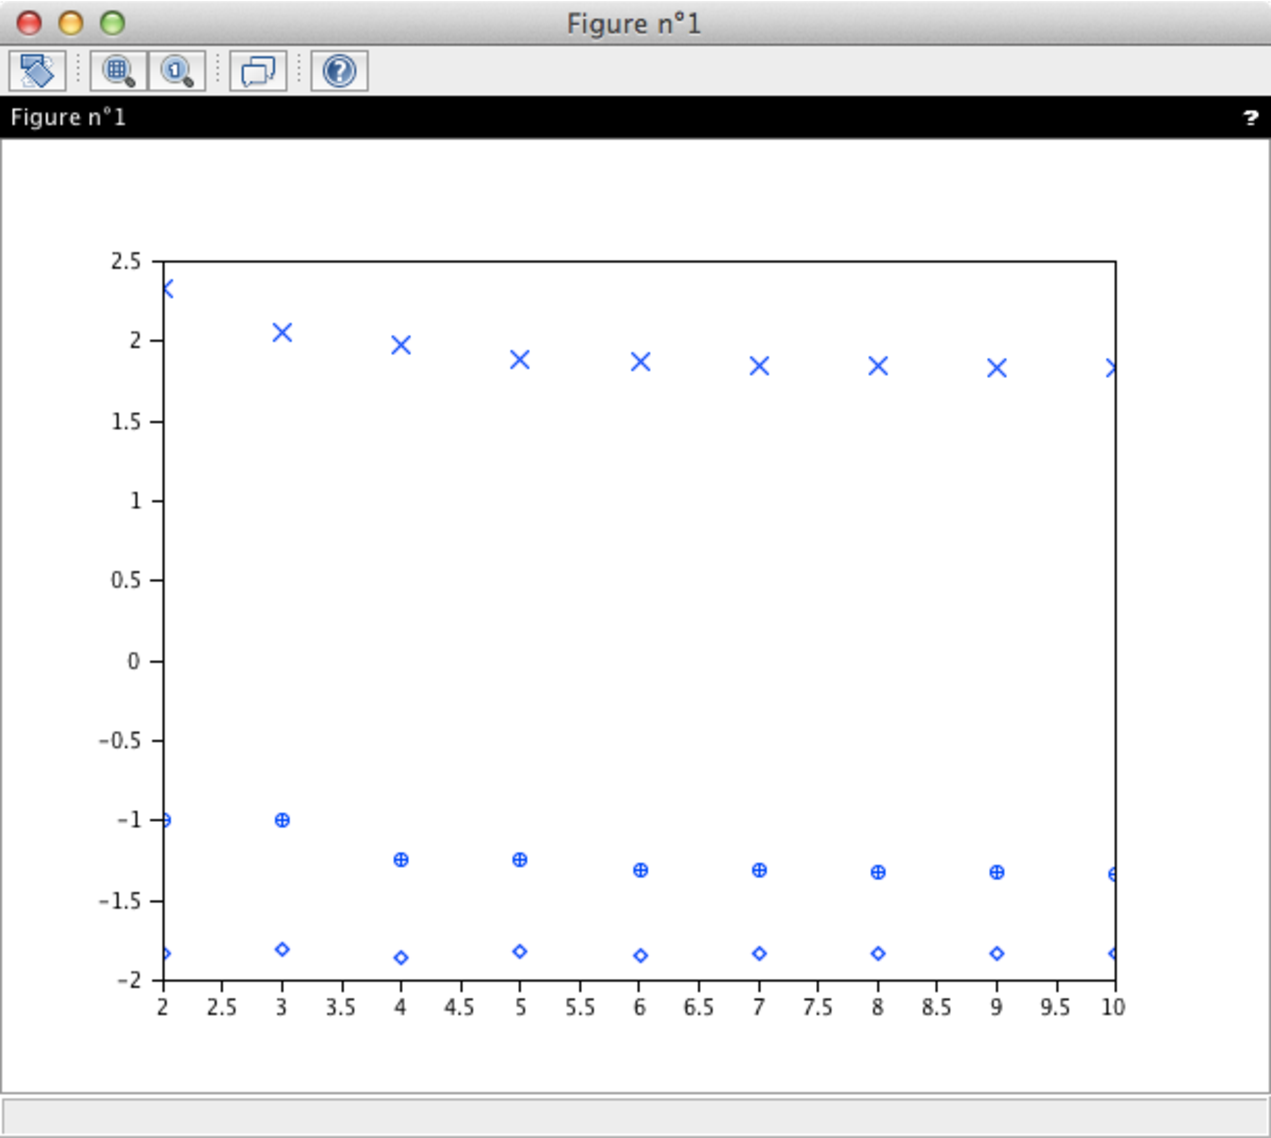
\includegraphics[width=10cm,
      height=8cm]{Figures/ECRICOME_2018/suites_alpha_beta_gamma.pdf}  
    \end{figure}
    % \caption{}
    % \label{fig:nuage}


    \newpage


    \begin{proof}~\\%
      Soit $n \in \N$.
      \begin{noliste}{$\sbullet$}
      \item D'après la question \itbf{5} :
        \[
        \beta_n = \left( \dfrac{1}{2} \right)^{n-1} - \dfrac{2}{3}
        \left(- \dfrac{1}{2} \right)^{n} - \dfrac{4}{3} \tendn
        -\dfrac{4}{3} \simeq -1,33
        \]
        En effet, comme $\left| \dfrac{1}{2} \right| < 1$ et $\left|
          -\dfrac{1}{2} \right| < 1$ alors : $\dlim{n \tend +\infty}
        \left( \dfrac{1}{2} \right)^{n-1} = 0$ \ et \ $\dlim{n \tend
          +\infty} \left( -\dfrac{1}{2} \right)^{n} = 0$.

      \item On démontre de même, toujours d'après les expressions
        obtenues en question \itbf{5.} : 
        \[
        \alpha_n \tendn \dfrac{11}{6} \simeq 1,8 \quad \text{ et }
        \quad \gamma_n \tendn -\dfrac{11}{6} \simeq -1,8
        \]

      \item Or, d'après la figure :
        \begin{noliste}{$\stimes$}
        \item la suite repérée par $\times$ semble converger vers un
          réel valant approximativement $1,8$.%
          \conc{Cette représentation graphique correspond à la suite
            $(\alpha_n)$.}
        \item la suite repérée par $\oplus$ semble converger vers un
          réel valant approximativement $-1,3$.%
          \conc{Cette représentation graphique correspond à la suite
            $(\beta_n)$.}
        \item la suite repérée par $\lozenge$ semble converger vers un
          réel valant approximativement $-1,8$.%
          \conc{Cette représentation graphique correspond à la suite
            $(\gamma_n)$.}
        \end{noliste}
      \end{noliste}
      \begin{remark}%L}{.97}%~%
        Il est possible de rédiger autrement.\\
        La représentation graphique commençant à $2$, on peut calculer
        :
        \[
        \alpha_2 = \dfrac{14}{6}, \quad \beta_2 = -1 \quad \text{ et }
        \quad \gamma_2 = -\dfrac{11}{6}
        \]
        ce qui permet d'associer chaque représentation graphique à la
        bonne suite.
      \end{remark}~\\[-1.2cm]
    \end{proof}
  \end{noliste}
\end{noliste}

\section*{Exercice 2}

\subsection*{Partie I : Étude de deux suites}

\noindent
Pour tout entier naturel $n$ non nul, on pose : \ $u_{n} = \Sum{k =
  1}{n} \dfrac{1}{k} - \ln(n)$ \ et \ $v_{n} = u_{n} - \dfrac{1}{n}$.

\begin{noliste}{1.}
 \setlength{\itemsep}{4mm}
\item Soit $f$ la fonction définie sur $\R_+^*$ par $f(x) =
  \dfrac{1}{x + 1} + \ln(x)-\ln(x + 1)$.
  \begin{noliste}{a)}
    \setlength{\itemsep}{2mm}
  \item Déterminer $ \dlim{x \to 0} f(x)$ et $ \dlim{x \to + \infty}
    f(x)$.

    \begin{proof}~%
      \begin{noliste}{$\sbullet$}
      \item Tout d'abord :
        \[
        \dfrac{1}{x + 1} \tendd{x}{0} \dfrac{1}{1} = 1, \quad \ln(x)
        \tendd{x}{0} -\infty \quad \text{ et } \quad \ln(x+1)
        \tendd{x}{0} \ln(1) = 0
        \]
        \conc{On en déduit $\dlim{x \tend 0} f(x) = -\infty$.}


        \newpage


      \item D'autre part : 
        \[
        \ln(x) - \ln(x+1) = - \big(\ln(x+1) - \ln(x) \big) = - \ln
        \left( \dfrac{x+1}{x} \right) = - \ln \left( 1 + \dfrac{1}{x}
        \right) \tendd{x}{+\infty} -\ln(1) = 0
        \]
        \conc{Comme de plus $\dfrac{1}{x + 1} \tendd{x}{+\infty} 0$,
          on en déduit $\dlim{x \tend +\infty} f(x) = 0$.}~\\[-1.2cm]
      \end{noliste}
    \end{proof}

  \item Étudier les variations de la fonction $f$ sur $\R_+^*$ et
    dresser son tableau de variations.

    \begin{proof}~%
      \begin{noliste}{$\sbullet$}
      \item La fonction $f$ est dérivable sur $]0, +\infty[$ comme
        somme de fonctions dérivables sur $]0, +\infty[$.

      \item Soit $x \in \ ]0, +\infty[$.
        \[
        \begin{array}{rcl}
          f'(x) & = & - \dfrac{1}{(x+1)^2} + \dfrac{1}{x} -
          \dfrac{1}{x+1} \\[.6cm]
          & = & \dfrac{-x + (x+1)^2 - x (x+1)}{x \ (x+1)^2}           
          \ = \ \dfrac{-x + (x^2 + 2x + 1) -x^2 - x}{x \ (x+1)^2} \ =
          \ \dfrac{1}{x \ (x+1)^2} 
        \end{array}
        \]
        Or $x (x+1)^2 > 0$. %
        \conc{Ainsi : $\forall x \in \ ]0, +\infty[$, $f'(x) > 0$.}~

      \item On en déduit le tableau de variations de $f$.\\[-.2cm]
        \begin{center}
          \begin{tikzpicture}[scale=0.8, transform shape]
            \tkzTabInit[lgt=4, espcl=5] %
            { %
              $x$ /1, %
              Signe de $f'(x)$ /1, %
              Variations de $f$ /2 } %
            {$0$, $+\infty$} %
            \tkzTabLine{ d , + , } %
            \tkzTabVar{D-/$-\infty$, +/$0$} %
          \end{tikzpicture}
        \end{center}
      \end{noliste}~\\[-1cm]
    \end{proof}

  \item Démontrer que : \ $\forall n \in \N^*, \ u_{n + 1}-u_{n} =
    f(n)$.

    \begin{proof}~\\%
      Soit $n \in \N^*$.
      \[
      \begin{array}{rcl}
        u_{n+1} - u_n & = & \left( \Sum{k=1}{n+1} \dfrac{1}{k} -
          \ln(n+1) \right) - \left( \Sum{k=1}{n} \dfrac{1}{k} -
          \ln(n) \right)
        \\[.6cm]
        & = & \left( \Sum{k=1}{n+1} \dfrac{1}{k} - \Sum{k=1}{n}
          \dfrac{1}{k} \right) - \ln(n+1) + \ln(n)
        \\[.6cm]
        & = & \dfrac{1}{n+1} + \ln(n) - \ln(n+1) \ = \ f(n)
      \end{array}
      \]
      \conc{$\forall n \in \N^*$, $u_{n+1} - u_n = f(n)$}~\\[-1cm]
    \end{proof}


    \newpage


  \item En déduire la monotonie de la suite $(u_{n})_{n\in \N^*}$.

    \begin{proof}~\\%
      Soit $n \in \N^*$.
      \begin{noliste}{$\sbullet$}
      \item D'après l'étude en question \itbf{1.b)}, la fonction $f$
        est strictement croissante sur $]0, +\infty[$ et de limite
        nulle en $+\infty$. On en déduit :
        \[
        \forall x \in \ ]0, +\infty[, f(x) < 0
        \]

      \item En appliquant cette propriété en $x = n$, on obtient,
        d'après la question précédente : 
        \[
        u_{n+1} - u_n = f(n) < 0
        \]
      \end{noliste}
      \conc{On en conclut que la suite $(u_n)_{n \in \N^*}$ est
        (strictement) décroissante.}~\\[-1cm]
    \end{proof}

  \item Écrire une fonction d'en-tête : {\tt function y = u(n)} qui
    prend en argument un entier naturel $n$ non nul et qui renvoie la
    valeur de $u_{n}$.

    \begin{proof}~%
      \begin{scilab}
        & \tcFun{function} \tcVar{y} = \underline{u}(\tcVar{n}) \nl %
        & \qquad S = 0 \nl %
        & \qquad \tcFor{for} k = 1:n \nl %
        & \qquad \qquad S = S + 1/k \nl %
        & \qquad \tcFor{end} \nl %
        & \qquad \tcVar{y} = S - log(\tcVar{n}) \nl %
        & \tcFun{endfunction}
      \end{scilab}
      Détaillons les différents éléments de ce code :
      \begin{noliste}{$\stimes$}
      \item en ligne \ligne{2}, on crée la variable {\tt S} dont le
        but est de contenir, en fin de programme $\Sum{k=1}{n}
        \frac{1}{k}$.\\
        Cette variable {\tt S} est donc initialisée à $0$.

      \item de la ligne \ligne{3} à la ligne \ligne{5}, on met à jour
        la variable {\tt S} à l'aide d'une boucle.\\
        Pour ce faire, on ajoute au $\eme{k}$ tour de boucle la
        quantité $\frac{1}{k}$.\\
        Ainsi, {\tt S} contient bien $\Sum{k=1}{n} \frac{1}{k}$ en
        sortie de boucle.

      \item en ligne \ligne{6}, on affecte à la variable {\tt y} la
        valeur $u_n = \Sum{k=1}{n} \frac{1}{k} - \ln(n)$.        
      \end{noliste}
      \begin{remark}%~
        Pour le calcul de la somme $\Sum{k=1}{n} \frac{1}{k}$, on peut
        aussi tirer profit des fonctionnalités \Scilab{} :\\%[-.2cm]
        \begin{scilabNC} 
          \qquad S = sum(1 ./ 1:n)
        \end{scilabNC}~\\[-.2cm]
        Pour bien comprendre cette instruction, rappelons que : 
        \begin{noliste}{$\stimes$}
        \item l'instruction {\tt 1:n} permet de créer la matrice ligne
          $(1 \quad 2 \quad \ldots \quad n)$.
        \item l'opérateur {\tt ./} permet d'effectuer la division
          terme à terme.\\
          Ainsi, l'instruction {\tt 1 ./ 1:n} permet de créer la
          matrice ligne $(\frac{1}{1} \quad \frac{1}{2} \quad \ldots
          \quad \frac{1}{n})$.
        \item la fonction {\tt sum} permet de sommer tous les
          coefficients d'une matrice.
        \end{noliste}
        On obtient donc bien la somme à calculer par cette méthode.
      \end{remark}~\\[-1.4cm]
    \end{proof}
  \end{noliste}


  \newpage


\item 
  \begin{noliste}{a)}
    \setlength{\itemsep}{2mm}
  \item Montrer que : $\forall n \in \N^*$, $v_{n + 1}-v_{n} =
    \dfrac{1}{n} - \ln \left(1 + \dfrac{1}{n} \right)$.

    \begin{proof}~\\%
      Soit $n \in \N^*$. Par définition :
      \[
      \begin{array}{rcl@{\quad}>{\it}R{4.6cm}}
        v_{n+1} - v_n & = & \left(u_{n+1} - \dfrac{1}{n+1} \right) -
        \left(u_{n} - \dfrac{1}{n} \right) 
        \\[.4cm]
        & = & (u_{n+1} - u_n) + \dfrac{1}{n} - \dfrac{1}{n+1}
        \\[.4cm]
        & = & \left(\bcancel{\dfrac{1}{n+1}} + \ln(n) - \ln(n+1) \right) +
        \dfrac{1}{n} - \bcancel{\dfrac{1}{n+1}}
        & (d'après la question \itbf{1.c)})
        \nl
        \nl[-.2cm]
        & = & \dfrac{1}{n} - \left(\ln(n+1) - \ln(n) \right) \ = \
        \dfrac{1}{n} - \ln\left( 1 + \dfrac{1}{n} \right)
      \end{array}
      \]
      \conc{$\forall n \in \N^*$, $v_{n + 1} - v_{n} = \dfrac{1}{n} -
        \ln \left(1 + \dfrac{1}{n} \right)$}~\\[-1cm]
    \end{proof}

  \item Montrer que pour tout réel $x$ positif : $\ln(1 + x) \leq x$.\\
    En déduire que la suite $(v_{n})_{n \in \N^*}$ est croissante.

    \begin{proof}~%
      \begin{noliste}{$\sbullet$}
      \item La fonction $g : x \mapsto \ln(x)$ est concave.\\
        On en déduit que sa courbe représentative ${\cal C}_f$ se
        situe sous ses tangentes, notamment celle au point d'abscisse
        $1$. Or cette tangente est la droite d'équation :
        \[
        \begin{array}{rcl}
          y & = & g(1) + g'(1) \ (x-1) 
          \\[.2cm]
          & = & \ln(1) + \dfrac{1}{1} \ (x-1) \ = \ x-1
        \end{array}
        \]
        On en déduit donc : 
        \[
        \forall x \in \ ]0, +\infty[, \ \ln(x) \ \leq \ x-1
        \]
        Soit $t \geq 0$. En appliquant la propriété ci-dessus à $x = 1
        + t \in \ ]0, +\infty[$, on obtient :
        \[
        \ln(1 + t) \leq (\bcancel{1}+t) - \bcancel{1} = t
        \]
        \conc{On a bien : $\forall t \geq 0$, $\ln(1+t) \leq t$.}
        \begin{remarkL}{.97}%~%
          \begin{noliste}{$\sbullet$}
          \item Notons tout d'abord que la variable $t$ étant sous la
            portée d'un quantificateur, elle est muette. Ainsi, le
            résultat démontré est bien celui souhaité.

          \item Il est possible de procéder différemment.\\
            On peut par exemple considérer la fonction $g_1 : x
            \mapsto \ln(1+x)$ et démontrer qu'elle est concave. Ainsi,
            la courbe ${\cal C}_{g_1}$ est située sous sa tangente au
            point d'abscisse $0$ :
            \[
            \forall x \geq 0, \ \ln(1 + x) \ \leq \ g_1(0) + g_1'(0) \
            (x-0) = \ln(1) + x = x
            \]

          \item On peut aussi considérer la fonction $g_2 : x \mapsto
            x - \ln(1+x)$, procéder à son étude et conclure quant à
            son signe :
            \[
            \forall x \geq 0, \ g_2(x) \geq 0
            \]
            ce qui correspond à l'inégalité souhaitée.
          \end{noliste}          
        \end{remarkL}


        \newpage


      \item Soit $n \in \N^*$. En appliquant l'inégalité précédente à
        $t = \dfrac{1}{n}$, on obtient :
        \[
        \ln\left( 1 + \dfrac{1}{n} \right) \leq \dfrac{1}{n} \quad
        \text{ et ainsi } \quad v_{n+1} - v_n = \dfrac{1}{n} -
        \ln\left( 1 + \dfrac{1}{n} \right) \geq 0
        \]
        \conc{On en déduit que la suite $(v_n)_{n \in \N^*}$ est
          croissante.}~\\[-1.4cm]
      \end{noliste}
    \end{proof}

  \item Donner le développement limité d'ordre 2 de $\ln(1 + x)$ en
    $0$. En déduire que :
    \[
    v_{n + 1}-v_{n} \underset{n\to + \infty}{\sim} \frac{1}{2n^{2}}
    \]
  \end{noliste}

  \begin{proof}~%
    \begin{noliste}{$\sbullet$}
    \item La fonction $h : x \mapsto \ln(1+x)$ est de classe
      $\Cont{2}$ sur l'intervalle $]-1, +\infty[$ car elle est la
      composée $h = h_2 \circ h_1$ où :
      \begin{noliste}{$\stimes$}
      \item $h_1 : x \mapsto 1 + x$ est :
        \begin{noliste}{$-$}
        \item de classe $\Cont{2}$ sur $]-1, +\infty[$ car
          polynomiale sur cet intervalle.
        \item telle que $h_1(]-1, +\infty[) \subset \ ]0, +\infty[$.
        \end{noliste}
      \item $h_2 : x \mapsto \ln(x)$ est de classe $\Cont{2}$ sur
        $]0, +\infty[$.
      \end{noliste}
      \concL{Ainsi, $h$ admet un développement limité d'ordre $2$ au
        voisinage de tout point de l'intervalle $]-1, +\infty[$ et
        donc en particulier de $0$.}{15}

    \item Ainsi, il existe une fonction $\eps$ définie dans un
      voisinage de $0$, telle que, au voisinage de $0$ :
      \[
      \begin{array}{rcl}
        h(x) & = & h(0) + h'(0) x + \dfrac{h''(0)}{2} x^2 + x^2 \
        \eps(x)
        \\[.2cm]
        & = & x - \dfrac{1}{2} \ x^2 + x^2 \ \eps(x)
      \end{array}
      \]
      où $\dlim{x \tend 0} \eps(x) = 0$.
    \item Comme $\dfrac{1}{n} \tendn 0$, on peut appliquer cette
      égalité à $x = \dfrac{1}{n}$ pour $n$ dans un voisinage de
      $+\infty$.\\
      On obtient :
      \[
      \ln\left( 1 + \dfrac{1}{n} \right) \ = \ \dfrac{1}{n} -
      \dfrac{1}{2} \ \dfrac{1}{n^2} + \dfrac{1}{n^2} \
      \eps\left( \dfrac{1}{n} \right)
      \]
      avec $\dlim{n \tend +\infty} \eps\left( \dfrac{1}{n} \right) =
      \dlim{x \tend 0} \eps(x) = 0$ par théorème de composition des
      limites.\\[.2cm]
      On peut donc écrire :
      \[
      v_{n} - v_{n+1} = \ln\left( 1 + \dfrac{1}{n} \right) -
      \dfrac{1}{n} \ = \ - \dfrac{1}{2} \ \dfrac{1}{n^2} +
      \oo{n}{+\infty}\left(\dfrac{1}{n^2} \right)
      \]
      \conc{Ainsi : $v_{n+1} - v_{n} = \dfrac{1}{2} \ \dfrac{1}{n^2} +
        \oo{n}{+\infty}\left(\dfrac{1}{n^2} \right)$ et donc $v_{n+1}
        - v_n \eqn{} \dfrac{1}{2n^2}$.}~\\[-1.2cm]
    \end{noliste}
  \end{proof}
  

  \newpage


  \begin{noliste}{a)}    
    \setcounter{enumii}{3}
  \item Déterminer la nature de la série de terme général $v_{n +
      1}-v_{n}$. On note $\gamma = \Sum{n = 1}{+ \infty}(v_{n +
      1}-v_{n})$.

    \begin{proof}~\\%
      D'après ce qui précède : 
      \begin{noliste}{$\stimes$}
      \item $v_{n+1} - v_n \eqn{} \dfrac{1}{2} \ \dfrac{1}{n^2}$.
      \item $\forall n \in \N^*$, $v_{n+1} - v_n \geq 0$ \ et \
        $\dfrac{1}{2} \ \dfrac{1}{n^2} \geq 0$.
      \item La série $\Sum{n \geq 1}{} \dfrac{1}{n^2}$ est convergente
        en tant que série de Riemann d'exposant $2$ ($> 1$).\\
        Il en est de même de la série $\Sum{n \geq 1}{} \dfrac{1}{2} \
        \dfrac{1}{n^2}$ (on ne change pas la nature d'une série en
        multipliant son terme général par un réel non nul).
      \end{noliste}
      \concL{Ainsi, par le critère d'équivalence des séries à termes
        positifs, la série $\Sum{n \geq 1}{} (v_{n+1} - v_n)$ est
        convergente.}{13}%~\\[-1cm]
      \begin{remark}%~%
        La seule difficulté de cette démonstration réside dans la
        rédaction du critère des séries à termes positifs (les
        arguments à utiliser ont tous été démontrés dans les questions
        précédentes). C'est donc une question d'application directe du
        cours qu'il convient de savoir traiter.
      \end{remark}~\\[-1.4cm]
    \end{proof}

  \item Pour $n \geq 2$, simplifier la somme partielle : \ $ \Sum{k =
      1}{n-1} (v_{k + 1}-v_{k})$.\\
    En déduire que la suite $(v_{n})_{n \geq 2}$ converge vers
    $\gamma$.

    \begin{proof}~\\%
      Soit $n \geq 2$.
      \begin{noliste}{$\sbullet$}
      \item Par sommation télescopique :
        \[
        \Sum{k=1}{n-1} (v_{k+1} - v_k) \ = \ v_{(n-1)+1} - v_1 \ = \
        v_n - v_1 
        \]
        On en déduit : $v_n = v_1 + \Sum{k=1}{n-1} (v_{k+1} - v_k)$.

      \item Or, d'après la question précédente, la série $\Sum{n \geq
          1}{} (v_{n+1} - v_n)$ est convergente.\\
        On déduit de l'écriture précédente de $v_n$ que la suite
        $(v_n)$ est convergente, de limite :
        \[
        \dlim{n \tend +\infty} v_n = v_1 + \Sum{k=1}{+\infty} (v_{k+1}
        - v_k) = v_1 + \gamma
        \]

      \item Enfin :
        \[
        v_1 = u_1 - \dfrac{1}{1} = \left(\Sum{k=1}{1} \dfrac{1}{k} -
          \bcancel{\ln(1)} \right) - 1 = 1 - 1 = 0
        \]
      \end{noliste}
      \conc{Ainsi, la suite $(v_n)$ est convergente, de limite
        $\dlim{n \tend +\infty} v_n = \gamma$.}
    \end{proof}

  \end{noliste}

\item 
  \begin{noliste}{a)} 
    \setlength{\itemsep}{2mm}
  \item Déterminer $ \dlim{n \to \infty} u_{n}$.

    \begin{proof}~\\%
      Soit $n \in \N^*$.\\
      Par définition : $u_n \ = \ v_n + \dfrac{1}{n}$.\\
      La suite $(u_n)_{n \in \N^*}$ est convergente car elle est la
      somme de suites convergentes.%
      \conc{De plus, $\dlim{n \tend +\infty} u_n = \dlim{n \tend
          +\infty} v_n + \dlim{n \tend +\infty} \dfrac{1}{n} = \gamma
        + 0 = \gamma$.}
      \begin{remarkL}{.97}%~
        \begin{noliste}{$\sbullet$}
        \item Il n’y a pas forcément dans les sujets une croissance
          linéaire de la difficulté. Au contraire, chaque nouvelle
          partie commence généralement par une question plus simple de
          mise en route. Il n’est donc pas judicieux de laisser de
          côté certaines parties.
        \item Cette question \itbf{3.a)} ne présente pas de
          difficulté. Comme dans la question \itbf{2.d)}, on est
          confronté ici à une question bilan qui consiste simplement à
          rappeler puis utiliser certains résultats précédents. Ces
          résultats étant fournis par l'énoncé, cette question peut
          être traitée même si les questions précédentes ne l'ont pas
          été.
        \end{noliste}
      \end{remarkL}~\\[-1.3cm]
    \end{proof}

  \item Montrer que :
    \[
    \forall n \in \N^*, \ v_{n} \leq \gamma \leq u_{n}
    \]
    puis que :
    \[
    \forall n \in \N^*, \ \big|u_{n} - \gamma\big| \leq \dfrac{1}{n}
    \]

    \begin{proof}~%
      \begin{noliste}{$\sbullet$}
      \item Dans ce qui précède, on a démontré que : 
        \begin{noliste}{$\stimes$}
        \item la suite $(v_n)_{n \in \N^*}$ est croissante (question
          \itbf{2.b}).
        \item la suite $(v_n)_{n \in \N^*}$ converge vers $\gamma$.
        \end{noliste}
        Démontrons alors que : $\forall n \in \N^*$, $v_n \leq
        \gamma$. Pour ce faire, on suppose par l'absurde que ce n'est
        pas le cas. Autrement dit, on suppose qu'il existe $n_0 \in
        \N^*$ tel que $v_{n_0} > \gamma$.\\[.2cm]
        La suite $(v_n)$ étant croissante : $\forall n \geq n_0, \ v_n
        \geq v_{n_0}$.\\
        Par passage à la limite dans cette inégalité, on obtient :
        $\gamma \geq v_{n_0}$.\\
        En combinant avec l'inégalité de l'hypothèse, on a alors :
        \[
        \gamma \geq v_{n_0} > \gamma
        \]
        Ce qui est absurde ! %
        \conc{On en conclut : $\forall n \in \N^*$, $v_n \leq \gamma$.}

      \item En appliquant le résultat précédent à la suite $(-u_n)_{n
          \in \N^*}$ qui est croissante (car $(u_n)_{n\in\N^*}$ est
        décroissante) et de limite $-\gamma$, on obtient :
        \[
        \forall n \in \N^*, \ -u_n \leq -\gamma
        \]
        \conc{Ainsi : $\forall n \in \N^*$, $u_n \geq \gamma$.}
      \end{noliste}

        \newpage


        \begin{remark}
          \begin{noliste}{$\sbullet$}
          \item L'esprit de l'énoncé semble être d'utiliser
            directement le résultat suivant :
            \[
            \Boxed{ %
              \left.
                \begin{array}{l}
                  \mbox{$(v_n)$ croissante} \\
                  v_n \tendn \ell
                \end{array}
              \right\} %
              \ \Rightarrow \ \mbox{$\forall n \in \N, \ v_n \leq
                \ell$}%
            }
            \]

          \item Le résultat encadré ci-dessus est lié à la notion de
            borne supérieure d'une suite, qui par définition, et sous
            réserve d'existence, est le plus petit des majorants de la
            suite. Si on connaît ce vocabulaire, on a accès à un
            énoncé plus précis du théorème de convergence monotone :
            toute suite croissante et majorée converge {\bf vers sa
              borne supérieure}. On peut alors démontrer le résultat
            précédent :
            \begin{noliste}{$\stimes$}
            \item la suite $(v_n)$ converge (vers $\ell$) donc elle
              est majorée,
            \item la suite $(v_n)$ est croissante.
            \end{noliste}
            Ainsi, d'après le théorème ci-dessus, $\ell = \dsup{n \in
              \N} v_n$ et donc : $\forall n \in \N$, $v_n \leq \ell$.
          \end{noliste}

        \end{remark}

        \begin{noliste}{$\sbullet$}
      \item Soit $n \in \N^*$. D'après l'inégalité précédente : $u_n -
        \gamma \geq 0$. On en déduit :
        \[
        \big| u_n - \gamma \big| \ = \ u_n - \gamma
        \]
        Or, par définition de la suite $(v_n)_{n \in \N^*}$ :
        \[
        u_n - \gamma \ = \ v_n + \dfrac{1}{n} - \gamma \ = \ \left(v_n
          - \gamma \right) + \dfrac{1}{n} \ \leq \ \dfrac{1}{n}
        \]
        car, d'après ce qui précède : $v_n - \gamma \leq 0$.%
        \conc{$\forall n \in \N^*$, $\big| u_n - \gamma \big| \ \leq \
          \dfrac{1}{n}$}~\\[-1.4cm]
      \end{noliste}
    \end{proof}

  \item On rappelle que l'instruction {\tt floor(x)} renvoie la partie
    entière d'un réel $x$ et on suppose que la fonction {\tt u} de la
    question \itbf{1.e)} a été correctement programmée. Expliquer
    l'intérêt et le fonctionnement du script ci-dessous :
    \begin{scilab}
      & eps = input(\ttq{}Entrer un réel strictement positif : \ttq{})
      \nl %
      & n = floor(1/eps) + 1 \nl %
      & disp(u(n))
    \end{scilab}

    \begin{proof}~%
      \begin{noliste}{$\sbullet$}
      \item Ce script a pour but d'afficher une valeur approchée de
        $\gamma$ à $\eps$ près (où $\eps$ est un réel strictement
        positif fourni par l'utilisateur et stocké dans la variable
        {\tt eps}).\\
        Pour ce faire, il faut commencer par trouver un entier $N \in
        \N^*$ tel que :
        \[
        \big| u_N - \gamma \big| \ \leq \ \eps
        \]
      \item Or, d'après ce qui précède : 
        \[
        \forall n \in \N^*, \ \big| u_n - \gamma \big| \ \leq \
        \dfrac{1}{n}
        \]
        Afin de trouver l'entier $N$ recherché, il suffit de trouver
        un entier $N \in \N^*$ tel que :
        \[
        \dfrac{1}{N} \ \leq \ \eps
        \]
        Si c'est le cas, on obtient alors, par transitivité :
        \[
        \big| u_N - \gamma \big| \ \leq \ \dfrac{1}{N} \ \leq \ \eps
        \]


        \newpage


      \item Raisonnons par équivalence pour trouver $N$ :
        \[
        \begin{array}{rcl@{\qquad}>{\it}R{5cm}}          
          \dfrac{1}{N} \ \leq \ \eps & \Leftrightarrow & N \ \geq \
          \dfrac{1}{\eps} & (par décroissance de la \\ fonction inverse
          sur $]0, +\infty[$)
        \end{array}
        \]
        Ainsi, tout entier plus grand que $\frac{1}{\eps}$
        convient. En particulier, l'entier $N = \lfloor \frac{1}{\eps}
        \rfloor + 1$ convient.
      \end{noliste}
      \conc{Ce script affiche la valeur $u_N$ où $N = \lfloor
        \frac{1}{\eps} \rfloor + 1$. C'est une valeur approchée de
        $\gamma$ à $\eps$ près.}~\\[-1.2cm]
    \end{proof}
  \end{noliste}
\end{noliste}

\section*{Partie II : Étude d'une série}

\noindent
Pour tout entier naturel $n$, on pose \ $a_{n} = \dfrac1{n(2n-1)}$.
\begin{noliste}{1.}
  \setlength{\itemsep}{4mm}
\item Démontrer que la série de terme général $a_{n}$ converge.

  \begin{proof}
    On a :
    \begin{noliste}{$\stimes$}
    \item $a_n = \dfrac{1}{n(2n-1)} \eqn{} \dfrac{1}{2} \
      \dfrac{1}{n^2}$.
    \item $\forall n \in \N^*$, $a_n \geq 0$ \ et \ $\dfrac{1}{2} \
      \dfrac{1}{n^2} \geq 0$.
    \item La série $\Sum{n \geq 1}{} \dfrac{1}{n^2}$ est convergente
      en tant que série de Riemann d'exposant $2$ ($> 1$).\\
      Il en est de même de la série $\Sum{n \geq 1}{} \dfrac{1}{2} \
      \dfrac{1}{n^2}$ (on ne change pas la nature d'une série en
      multipliant son terme général par un réel non nul).
    \end{noliste}
    \conc{Ainsi, par le critère d'équivalence des séries à termes
      positifs, la série $\Serie a_n$ est convergente.}
    \begin{remark}%~
      La démonstration demandée ici est à peu de choses près celle de
      la question \itbf{I.2.d)}.
    \end{remark}~\\[-1.2cm]
  \end{proof}

\item
  \begin{noliste}{a)} 
    \setlength{\itemsep}{2mm}
  \item Justifier que : $\forall n \in \N^*, \ \Sum{k = 1}{n}
    \dfrac{1}{2k-1} = \Sum{k = 1}{2n} \dfrac{1}{k} - \Sum{k = 1}{n}
    \dfrac{1}{2k}$.
    
    \begin{proof}~\\%
      Soit $n \in \N^*$. Remarquons :
      \[
      \begin{array}{rcccc}
        \Sum{k = 1}{2n} \dfrac{1}{k} & = & \Sum{ %
          \scalebox{.8}{$
            \begin{array}{c}
              k \in \llb 1, 2n \rrb \\
              \text{$k$ pair}
            \end{array}
            $} }{} \dfrac{1}{k}
        & + & \Sum{ %
          \scalebox{.8}{$
            \begin{array}{c}
              k \in \llb 1, 2n \rrb \\
              \text{$k$ impair}
            \end{array}
            $} }{} \dfrac{1}{k} 
        \\[.6cm]
        & = & 
        \left(
          \dfrac{1}{2} + \dfrac{1}{4} + \ldots + \dfrac{1}{2n}            
        \right)
        & + & 
        \left(
          \dfrac{1}{1} + \dfrac{1}{3} + \ldots + \dfrac{1}{2n-1}            
        \right)
        \\[.4cm]
        & = & \Sum{i=1}{n} \dfrac{1}{2i} 
        & + & \Sum{i=1}{n} \dfrac{1}{2i-1} 
      \end{array}
      \]
      \conc{$\forall n \in \N^*, \ \Sum{k = 1}{n} \dfrac{1}{2k-1} =
        \Sum{k = 1}{2n} \dfrac{1}{k} - \Sum{k = 1}{n} \dfrac{1}{2k}$.}
      \begin{remarkL}{.97}%~%
        \begin{noliste}{$\sbullet$}
        \item L'énoncé demande de \og Justifier \fg{} le
          résultat. Cette terminologie est souvent associée à des
          démonstrations courtes et éventuellement moins formelles.

        \item Il est aussi possible ici de procéder par
          récurrence. Détaillons la rédaction.\\[.2cm]
          Démontrons par récurrence : $\forall n \in \N^*$, $\PP{n}$
          \quad où \quad $\PP{n}$ : $\Sum{k = 1}{n} \dfrac{1}{2k-1} =
          \Sum{k = 1}{2n} \dfrac{1}{k} - \Sum{k = 1}{n}
          \dfrac{1}{2k}$.
          \begin{noliste}{\fitem}
          \item {\bf Initialisation} :
          \end{noliste}
          \begin{liste}{$-$}
          \item D'une part : $\Sum{k = 1}{1} \dfrac{1}{2k-1} =
            \dfrac{1}{2-1} = \dfrac{1}{1} = 1$.
          \item D'autre part : $\Sum{k = 1}{2} \dfrac{1}{k} - \Sum{k
              = 1}{1} \dfrac{1}{2k} = \left( \dfrac{1}{1} +
              \bcancel{\dfrac{1}{2}} \right) -
            \bcancel{\dfrac{1}{2}} = 1$.
          \item[] D'où $\PP{0}$.
          \end{liste}          
          
          \begin{noliste}{\fitem}
          \item {\bf Hérédité} : soit $n \in \N^*$.\\
            Supposons $\PP{n}$ et démontrons $\PP{n+1}$ %
            $\left(
              \begin{array}{l}
                \text{\ie } \ \Sum{k =
                  1}{n+1} \dfrac{1}{2k-1} = \Sum{k = 1}{2(n+1)} \dfrac{1}{k} -
                \Sum{k = 1}{n+1} \dfrac{1}{2k}
              \end{array}
            \right)$.\\[-.1cm]
            \[
            \begin{array}{rcl@{\qquad}>{\it}R{3.5cm}}
              \Sum{k=1}{n+1} \dfrac{1}{2k-1} & = & \left(\Sum{k=1}{n}
                \dfrac{1}{2k-1} \right) + \dfrac{1}{2(n+1)-1}
              \\[.6cm]
              & = & \left( \Sum{k=1}{2n} \dfrac{1}{k} - \Sum{k = 1}{n}
                \dfrac{1}{2k} \right) + \dfrac{1}{2n+1} & (par hypothèse \\
              de récurrence)
              \nl
              \nl[-.2cm]
              & = & \Sum{k=1}{2n+1} \dfrac{1}{k} - \Sum{k = 1}{n}
              \dfrac{1}{2k} 
              \\[.6cm]
              & = & \left( \Sum{k=1}{2n+1} \dfrac{1}{k} + \dfrac{1}{2n+2}
              \right) - \left( \Sum{k = 1}{n} \dfrac{1}{2k} +
                \dfrac{1}{2n+2} \right) 
              & (en introduisant $\dfrac{1}{2n+2} - \dfrac{1}{2n+2}$)
              \nl
              \nl[-.2cm]
              & = & \Sum{k=1}{2n+2} \dfrac{1}{k} - \Sum{k = 1}{n+1}
              \dfrac{1}{2k} 
            \end{array}
            \]
            D'où $\PP{n+1}$.
          \end{noliste}
          \conc{Ainsi, par principe de récurrence : $\forall n \in
            \N^*$, $\PP{n}$.}
        \end{noliste}

      \end{remarkL}~\\[-1.4cm]
    \end{proof}

  \item Déterminer deux réels $\alpha$ et $\beta$ tels que : $\forall
    n \in \N^*, \ a_{n} = \dfrac{\alpha}{n} + \dfrac{\beta}{2n-1}$.

    \begin{proof}~\\%
      Soit $n \in \N^*$. On raisonne par équivalence.
      \[
      \begin{array}{cl@{\quad}>{\it}R{3.5cm}}        
        & a_{n} = \dfrac{\alpha}{n} + \dfrac{\beta}{2n-1} 
        \\[.6cm]
        \Leftrightarrow & \dfrac{1}{n(2n-1)} = \dfrac{\alpha \ (2n-1)
          + \beta \ n}{n(2n-1)}   
        \\[.6cm]
        \Leftrightarrow & \dfrac{1}{n(2n-1)} = \dfrac{(2 \alpha +
          \beta) \ n - \alpha}{n(2n-1)}   
        \\[.6cm]
        \Leftrightarrow & 1 = (2 \alpha + \beta) \ n - \alpha
        & (en multipliant par $n(2n-1) > 0$)
      \end{array}
      \]


      \newpage


      \noindent 
      La dernière égalité étant vérifiée pour tout entier non nul $n$,
      elle est équivalente, par identification, au système suivant :
      \[
      (S)
      \left\{
        \begin{array}{rcrcr}
          2 \alpha & + & \beta & = & 0 \\
          - \alpha & & & = & 1
        \end{array}
      \right.
      \]
      Et enfin : $(S)
      \begin{arrayEq}
        L_1 \leftarrow L_1 + 2 \ L_2
      \end{arrayEq}
      \left\{
        \begin{array}{rcrcr}
          & & \beta & = & 2 \\
          - \alpha & & & = & 1
        \end{array}
      \right.
      $. %
      \conc{Les réels $\alpha = -1$ et $\beta = 2$ conviennent.}~\\[-1cm]
    \end{proof}

  \item En déduire que : $\forall n \in \N^*$, $\Sum{k = 1}{n} a_{k} =
    2 \Sum{k = n + 1}{2n} \dfrac{1}{k}$.

    \begin{proof}~\\%
      Soit $n \in \N^*$.
      \begin{noliste}{$\sbullet$}
      \item D'après la question précédente, pour tout $k \in \N^*$ :
        \[
        a_k \ = \ \dfrac{-1}{k} + \dfrac{2}{2k-1}
        \]
      \item En sommant ces égalités membre à membre, on obtient, par
        linéarité de la somme :
        \[
        \begin{array}{rcl@{\qquad}>{\it}R{3.5cm}}
          \Sum{k=1}{n} a_k & = & \Sum{k=1}{n} \dfrac{-1}{k} +
          \Sum{k=1}{n} \dfrac{2}{2k-1}
          \\[.6cm]
          & = & \Sum{k=1}{n} \dfrac{-1}{k} + 2 \ \Sum{k=1}{n} \dfrac{1}{2k-1}
          \\[.6cm]
          & = & \Sum{k=1}{n} \dfrac{-1}{k} + 2 \ \left( \Sum{k =
              1}{2n} \dfrac{1}{k} - \Sum{k = 1}{n} \dfrac{1}{2k}
          \right)
          & (d'après la \\ question \itbf{2.b)})
          \nl 
          \nl[-.2cm]
          & = & \Sum{k=1}{n} \dfrac{-1}{k} + 2 \ \Sum{k=1}{2n}
          \dfrac{1}{k} - \bcancel{2} \ \Sum{k = 1}{n}
          \dfrac{1}{\bcancel{2}k}
          \\[.6cm]
          & = & 2 \ \Sum{k=1}{2n} \dfrac{1}{k} + \left( \Sum{k=1}{n}
            \dfrac{-1}{k} - \Sum{k=1}{n} \dfrac{1}{k} \right)
          \\[.6cm]
          & = & 2 \ \Sum{k=1}{2n} \dfrac{1}{k} - 2 \Sum{k=1}{n}
          \dfrac{1}{k} \ = \ 2 \ \left( \Sum{k=1}{2n} \dfrac{1}{k} -
            \Sum{k=1}{n} \dfrac{1}{k} \right) 
          \\[.6cm]
          & = & 2 \ \left( \bcancel{\Sum{k=1}{n} \dfrac{1}{k}} +
            \Sum{k=n+1}{2n} \dfrac{1}{k} - \bcancel{\Sum{k=1}{n}
              \dfrac{1}{k}} \right) \ = \ 2 \Sum{k=n+1}{2n} \dfrac{1}{k}
        \end{array}
        \]        
      \end{noliste}
      \conc{$\forall n \in \N^*$, $\Sum{k=1}{n} a_k \ = \ 2
        \Sum{k=n+1}{2n} \dfrac{1}{k}$}~\\[-1cm]
    \end{proof}
  \end{noliste}


  \newpage


\item 
  \begin{noliste}{a)}
    \setlength{\itemsep}{2mm}
  \item Montrer que : 
    \[
    \forall n \in \N^*, \ \Sum{k = n + 1}{2n} \dfrac{1}{k} =
    u_{2n}-u_{n} + \ln(2)
    \]
    où $(u_{n})_{n \in \N^*}$ est la suite définie dans la partie I.

    \begin{proof}~\\%
      Soit $n \in \N^*$. Par définition de la suite $(u_n)_{n \in
        \N^*}$ :
      \[
      \begin{array}{rcl@{\quad}>{\it}R{3.5cm}}
        u_{2n} - u_n & = & \left( \Sum{k=1}{2n} \dfrac{1}{k} - \ln(2n)
        \right) - \left( \Sum{k=1}{n} \dfrac{1}{k} - \ln(n) \right) 
        \\[.6cm]
        & = & \left( \Sum{k=1}{2n} \dfrac{1}{k} - \Sum{k=1}{n}
          \dfrac{1}{k} \right) - \left( \ln(2n)  - \ln(n) \right) 
        \\[.6cm]
        & = & \Sum{k=n+1}{2n} \dfrac{1}{k} - \big( (\ln(2) +
        \bcancel{\ln(n)} )  - \bcancel{\ln(n)} \big) \ = \
        \Sum{k=n+1}{2n} \dfrac{1}{k} - \ln(2)
      \end{array}
      \]
      \conc{On en déduit, en réordonnant : $\forall n \in \N^*$,
        $\Sum{k=n+1}{2n} \dfrac{1}{k} = u_{2n} -u_n + \ln(2)$.}~\\[-1cm]
    \end{proof}

  \item Calculer alors  $\Sum{k = 1}{+ \infty} a_{k}$.
    
    \begin{proof}~%
      \begin{noliste}{$\sbullet$}
      \item D'après la question \itbf{1.}, la série $\Serie a_n$ est
        convergente.

      \item Déterminons sa somme. Soit $n \in \N^*$.
        \[
        \begin{array}{rcl@{\qquad}>{\it}R{5cm}}
          \Sum{k=1}{n} a_k & = & 2 \ \Sum{k=n+1}{2n} \dfrac{1}{k} 
          & (d'après la question \itbf{2.c)})
          \nl
          \nl[-.2cm]
          & = & 2 \ \left(  u_{2n} -u_n + \ln(2) \right)
          & (d'après la question \itbf{3.a)})
          \nl
          \nl[-.2cm]
          & \tendn & 2 \ (\bcancel{\gamma} - \bcancel{\gamma} + \ln(2))
          & (car comme la suite $(u_n)$ converge vers $\gamma$, il en
          est de même de sa sous-suite $(u_{2n})$)
        \end{array}
        \]
      \end{noliste}
      \conc{On en conclut : $\Sum{k=1}{+\infty} a_k = 2 \ln(2)$.}~\\[-1cm]
    \end{proof}
  \end{noliste}

\item 
  \begin{noliste}{a)}
    \setlength{\itemsep}{2mm}
  \item Montrer que : $\forall n \in \N^*, \ \Sum{k = n + 1}{2n}
    \dfrac{1}{k} = \dfrac{1}{n} \ \Sum{k = 1}{n} \dfrac{1}{1 +
      \frac{k}{n}}$.

    \begin{proof}~\\%
      Soit $n \in \N^*$.
      \[
      \begin{array}{rcl@{\quad}>{\it}R{4.5cm}}
        \Sum{k = n + 1}{2n} \dfrac{1}{k} & = & \Sum{k = 1}{n}
        \dfrac{1}{k + n} 
        & (par décalage d'indice) 
        \nl
        \nl[-.2cm]
        & = & \Sum{k = 1}{n} \dfrac{1}{n \left( \frac{k}{n} + 1
          \right)} 
        \ = \ \dfrac{1}{n} \ \Sum{k = 1}{n} \dfrac{1}{1 + \frac{k}{n}} 
      \end{array}
      \]
      \conc{$\forall n \in \N^*, \ \Sum{k = n + 1}{2n} \dfrac{1}{k} =
        \dfrac{1}{n} \ \Sum{k = 1}{n} \dfrac{1}{1 + \frac{k}{n}}$}~\\[-1cm]
    \end{proof}


    \newpage


  \item Retrouver alors le résultat de la question \itbf{3.b)}.

    \begin{proof}~%
      \begin{noliste}{$\sbullet$}
      \item D'après la question précédente :
        \[
        \Sum{k = n + 1}{2n} \dfrac{1}{k} \ = \ \dfrac{1}{n} \ \Sum{k =
          1}{n} \dfrac{1}{1 + \frac{k}{n}} \ = \ \dfrac{1}{n} \ \Sum{k
          = 1}{n} f\left( \dfrac{k}{n} \right)
        \]
        où la fonction $f : x \mapsto \dfrac{1}{1+x}$ est continue sur
        $[0, 1]$.

      \item On reconnaît une somme de Riemann, ce qui démontre :
        \[
        \dfrac{1}{n} \ \Sum{k = 1}{n} f\left( \dfrac{k}{n} \right)
        \tendn \dint{0}{1} f(x) \dx
        \]
        Or :
        \[
        \dint{0}{1} f(x) \dx \ = \ \dint{0}{1} \dfrac{1}{1+x} \dx \ =
        \ \Prim{\ln\big( |1+x| \big)}{0}{1} \ = \ \Prim{\ln\big( 1+x
          \big)}{0}{1} \ = \ \ln(2) - \bcancel{\ln(1)}
        \]

      \item Ainsi, d'après la question \itbf{2.c)} :
        \[
        \Sum{k = 1}{n} a_k \ = \ 2 \ \Sum{k = n + 1}{2n} \dfrac{1}{k}
        \tendn 2 \ \ln(2)
        \]
      \end{noliste}
      \conc{On retrouve bien : $\Sum{k = 1}{+\infty} a_k = 2 \
        \ln(2)$}~\\[-1cm] 
    \end{proof}

  \end{noliste}
\end{noliste}

\section*{Exercice 3}

\noindent
Soit $n$ un entier naturel non nul.\\
Dans une fête foraine, un stand propose le jeu suivant : le joueur
lance $n$ fois une pièce et compte le nombre de Pile obtenus. Si ce
nombre est pair, le joueur est déclaré vainqueur, et s'il est impair,
il est déclaré perdant.\\
Si le joueur est déclaré vainqueur, il gagne 10 euros pour chaque Pile
obtenu, mais s'il a perdu, il doit payer 10 euros pour chaque Pile
obtenu.\\
En particulier, s'il n'obtient aucun Pile, il est déclaré vainqueur,
mais ne remporte rien. La pièce est truquée, et à chaque lancer, la
probabilité d'obtenir Pile est égale à $p$ ($p \in \ ]0,1[$), et celle
d'obtenir Face est de $1-p$.\\
On notera $X$ la variable aléatoire égale au nombre de Pile obtenus,
et $G$ la variable aléatoire égale au gain algébrique du joueur.\\
Enfin, on notera $A$ l'événement : \og le joueur est déclaré
vainqueur \fg{} et on dira que le jeu est favorable au joueur si
l'espérance mathématique de la variable aléatoire $G$ est positive.



\newpage


\subsection*{Partie I}
 
\noindent
Dans cette partie, on suppose que $n = 3$ et $p = \dfrac{2}{3}$.
\begin{noliste}{1.}
  \setlength{\itemsep}{4mm}
\item Reconnaître la loi de $X$ et vérifier que : $\Prob\left(A\right)
  = \dfrac{13}{27}$.

  \begin{proof}~%
    \begin{noliste}{$\sbullet$}
    \item Commençons par décrire l'expérience.
      \begin{noliste}{$-$}
      \item Chaque lancer de pièce est une épreuve à deux issues :
        Pile (issue nommée succès), obtenu avec la probabilité $p$ et
        Face, obtenu avec la probabilité $1 - p$.
      \item Ainsi, l'expérience consiste en la succession de $n$
        épreuves de Bernoulli indépendantes et de même paramètre $p$.
      \end{noliste}
      La \var $X$ compte le nombre de succès obtenu au cours de cette
      expérience.%
      \conc{Ainsi : $X \suit \Bin{n}{p}$.}

    \item L'événement $A$ est réalisé si et seulement si le joueur a
      obtenu un nombre pair de Pile.\\
      Comme $n = 3$, ceci ne se produit que si le joueur n'obtient
      aucun Pile ou en obtient deux.\\
      On en déduit :
      \[
      A \ = \ \Ev{X = 0} \ \cup \ \Ev{X=2}
      \]
      Ainsi, en appliquant $\Prob$ de part et d'autre : 
      \[
      \begin{array}{rcl@{\quad}>{\it}R{4.5cm}}
        \Prob(A) & = & \Prob\big( \Ev{X = 0} \ \cup \ \Ev{X=2} \big)
        \\[.2cm]
        & = & \Prob\big( \Ev{X = 0} \big) + \Prob\big( \Ev{X=2} \big)
        & (car $\Ev{X = 0}$ et $\Ev{X=2}$ \\ sont incompatibles)
        \nl
        \nl[-.4cm]
        & = & \dbinom{3}{0} \ p^0 (1-p)^3 + \dbinom{3}{2} \ p^2
        (1-p)^1
        & (car $X \suit \Bin{3}{p}$)
        \nl
        \nl[-.2cm]
        & = & \left(\dfrac{2}{3} \right)^0 \ \left(\dfrac{1}{3}
        \right)^3 + 3 \ \left(\dfrac{2}{3} \right)^2 
        \left(\dfrac{1}{3} \right)
        & (car $p = \dfrac{2}{3}$)
        \nl
        \nl[-.2cm]
        & = & \dfrac{1}{27} + 3 \ \dfrac{4}{27} \ = \ \dfrac{13}{27}
      \end{array}
      \]
    \end{noliste}
    \conc{On obtient bien : $\Prob(A) = \dfrac{13}{27}$.}~\\[-.8cm]
  \end{proof}

\item Montrer que : $G(\Omega) = \{-30, -10, 0, 20\}$, puis expliciter
  la loi de $G$.

  \begin{proof}~%
    \begin{noliste}{$\sbullet$}
    \item Le gain du joueur dépend du nombre de Pile obtenus : 
      \begin{noliste}{$\stimes$}
      \item \dashuline{si le joueur obtient $0$ Pile}, il est déclaré
        vainqueur et touche : $0 \times 10 = 0$ euros.

      \item \dashuline{si le joueur obtient $1$ Pile}, il est déclaré
        perdant et touche : $1 \times (-10) = -10$ euros.

      \item \dashuline{si le joueur obtient $2$ Pile}, il est déclaré
        vainqueur et touche : $2 \times 10 = 20$ euros.

      \item \dashuline{si le joueur obtient $3$ Pile}, il est déclaré
        perdant et touche : $3 \times (-10) = -30$ euros.
      \end{noliste}
      \conc{Ainsi, $G(\Omega) = \{-30, -10, 0, 20\}$.}
      \begin{remark}%~
        La variable $G$ représente le gain {\bf algébrique} du
        joueur. Cela signifie que $G$ peut prendre des valeurs
        positives (en cas de victoire du joueur) ou négatives (en cas
        de défaite). Si le gain algébrique du joueur est de $-30$,
        cela signifie que le joueur doit payer $30$ euros.
      \end{remark}


      \newpage


    \item D'après ce qui précède : 
      \[
      \begin{array}{lcl}
        \Prob\big(\Ev{G = 0} \big) & = & \Prob\big( \Ev{X = 0} \big) \ = \
        \dbinom{3}{0} \ p^0 (1-p)^3 \ = \ \left( \dfrac{1}{3} \right)^3 \ = \
        \dfrac{1}{27}
        \\[.6cm]
        \Prob\big(\Ev{G = -10} \big) & = &  \Prob\big( \Ev{X = 1} \big) \ = \
        \dbinom{3}{1} \ p^1 (1-p)^2 \ = \ 3 \ \dfrac{2}{3} \ \left(
          \dfrac{1}{3} \right)^2 \ = \ \dfrac{6}{27}
        \\[.6cm]
        \Prob\big(\Ev{G = 20} \big) & = & \Prob\big( \Ev{X = 2} \big) \ = \
        \dbinom{3}{2} \ p^2 (1-p)^1 \ = \ 3 \ \left( \dfrac{2}{3} \right)^2
        \ \left( \dfrac{1}{3} \right)^1 \ = \ \dfrac{12}{27}
        \\[.6cm]
        \Prob\big(\Ev{G = -30} \big) & = & \Prob\big( \Ev{X = 3} \big) \ = \
        \dbinom{3}{3} \ p^3 (1-p)^0 \ = \ \left( \dfrac{2}{3} \right)^3 \ = \
        \dfrac{8}{27}
      \end{array}
      \]
      \conc{$\Prob\big( \Ev{G = -30}\big) = \dfrac{8}{27}$, \
        $\Prob\big( \Ev{G = -10}\big) = \dfrac{6}{27}$, \ $\Prob\big(
        \Ev{G = 0}\big) = \dfrac{1}{27}$, \ $\Prob\big( \Ev{G = 20
        }\big) = \dfrac{12}{27}$}
    \end{noliste}    
    \begin{remark}%~
      \begin{noliste}{$\sbullet$}
      \item Dans cette question, on calcule $\Prob\big( \Ev{G = x}
        \big)$ pour tout $x \in G(\Omega)$. On peut s'affranchir du
        dernier calcul (à savoir $\Prob\big( \Ev{G = -30} \big)$),
        puisque, comme $\Big( \Ev{G = x} \Big)_{x \in \{-30, -10, 0,
          20\}}$ est un système complet d'événements, on a :
        \[
        \Prob\big(\Ev{G = 0} \big) + \Prob\big(\Ev{G = -10} \big) +
        \Prob\big(\Ev{G = 20} \big) + \Prob\big(\Ev{G = -30} \big) = 1
        \]
        et donc :
        \[
        \Prob\big(\Ev{G = -30} \big) = 1 - \Prob\big(\Ev{G = 0} \big)
        - \Prob\big(\Ev{G = -10} \big) - \Prob\big(\Ev{G = 20} \big) 
        \]
      \item Toutefois, il est vivement conseillé de réaliser tous ces
        calculs et d'utiliser la propriété ci-dessus comme mesure de
        vérification.
      \end{noliste}
    \end{remark}~\\[-1.4cm]
  \end{proof}

\item Calculer l'espérance de $G$. Le jeu est-il favorable au joueur ?
  
  \begin{proof}~%
    \begin{noliste}{$\sbullet$}
    \item La \var $G$ admet une espérance car c'est une \var finie.

    \item Par définition :
      \[
      \begin{array}{rcl}
        \E(G) & = & \Sum{x \in G(\Omega)}{} x \ \Prob\big( \Ev{G = x} \big) 
        \\[.6cm]
        & = & -30 \ \Prob\big( \Ev{G = -30} \big) - 10 \ \Prob\big(
        \Ev{G = -10} \big) + 0 \ \Prob\big( \Ev{G = 0} \big) + 20 \
        \Prob\big( \Ev{G = 20} \big) 
        \\[.2cm]
        & = & -30 \ \dfrac{8}{27} - 10 \ \dfrac{6}{27} + 20 \
        \dfrac{12}{27}
        \\[.6cm]
        & = & \dfrac{-\bcancel{240} - 60 + \bcancel{240}}{27} 
        \\[.4cm]
        & = & \dfrac{-60}{27} \ = \ -\dfrac{20}{9}
      \end{array}
      \]      
    \end{noliste}
    \conc{L'espérance de gain est négative donc le jeu n'est pas
      favorable au joueur.}%
    {\it (le joueur perd en moyenne environ $2,22$ euros par partie)}~\\[-.4cm]
  \end{proof}
\end{noliste}


\newpage


\subsection*{Partie II}

\noindent
Dans cette partie, on revient au cas général, où $n$ est entier
naturel non nul et $p \in \ ]0,1[$.\\
Celui qui tient le stand souhaite rendre le jeu plus attractif en
affichant \og À ce jeu, il y a plus de gagnants que de perdants ! \fg,
et cherche donc les conditions nécessaires sur $p$ et $n$ pour que son
affichage ne soit pas mensonger.\\
Soit $Y$ la variable aléatoire définie par : $Y = (-1)^{X}$.\\
Autrement dit, $Y$ prend la valeur $1$ lorsque $X$ prend une valeur
paire, et $Y$ prend la valeur $-1$ lorsque $X$ prend une valeur
impaire.
\begin{noliste}{1.}
  \setlength{\itemsep}{4mm}
\item
  \begin{noliste}{a)} 
    \setlength{\itemsep}{2mm}
  \item On note $Z = \dfrac{Y + 1}{2}$.\\[.2cm]
    Déterminer $Y(\Omega)$, puis montrer que $Z$ suit une loi de
    Bernoulli de paramètre $\Prob\left( A \right)$.

    \begin{proof}~%
      \begin{noliste}{$\sbullet$}
      \item Soit $\omega \in \Omega$. Deux cas se présentent.
        \begin{noliste}{$\stimes$}
        \item \dashuline{Si $X(\omega)$ est pair} : alors $Y(\omega) =
          (-1)^{X(\omega)} = 1$. Et dans ce cas :
          \[
          Z(\omega) \ = \ \dfrac{Y(\omega) + 1}{2} \ = \ \dfrac{2}{2}
          \ = \ 1
          \]
        \item \dashuline{Si $X(\omega)$ est impair} : alors $Y(\omega)
          = (-1)^{X(\omega)} = -1$.  Et dans ce cas :
          \[
          Z(\omega) \ = \ \dfrac{Y(\omega) + 1}{2} \ = \ \dfrac{0}{2}
          \ = \ 0
          \]
        \end{noliste}
        \conc{$Y(\Omega) = \{-1, 1\}$ \quad et \quad $Z(\Omega) = \{0,
          1\}$}

      \item Comme $Z(\Omega) = \{0, 1\}$, la \var $Z$ suit une loi de
        Bernoulli dont le paramètre vaut :
        \[
        \Prob\big( \Ev{Z = 1} \big) \ = \ \Prob\big( \Ev{Y = 1} \big)
        \ = \ \Prob\big( \Ev{\text{$X$ est pair}} \big) \ = \ \Prob(A)
        \]
        \conc{$Z \suit \Bern{\Prob(A)}$}~\\[-1.2cm]
      \end{noliste}
    \end{proof}

  \item Démontrer que : $\E(Y) = 2 \Prob(A) - 1$.

    \begin{proof}~%
      \begin{noliste}{$\sbullet$}
      \item La \var $Y$ admet une espérance car elle est finie.\\
        Par définition :
        \[
        \begin{array}{rcl}
          \E(Y) & = & \Sum{y \in Y(\Omega)}{} y \ \Prob\big( \Ev{Y =
            y} \big)
          \\[.6cm]
          & = & (-1) \times \Prob\big( \Ev{Y = -1} \big) + 1 \times
          \Prob\big( \Ev{Y = 1} \big) 
          \\[.2cm]
          & = & (-1) \times \left( 1 - \Prob\big( \Ev{Y = 1} \big)
          \right) + \Prob\big( \Ev{Y = 1} \big) 
          \\[.2cm]
          & = & (-1) \times \left( 1 - \Prob(A) \right) + \Prob(A) 
          \\[.2cm]
          & = & 2 \Prob(A) - 1
        \end{array}
        \]
      \end{noliste}
      \conc{$\E(Y) \ = \ 2 \Prob(A) - 1$}~\\[-1cm]
    \end{proof}
  \end{noliste}


  \newpage


\item 
  \begin{noliste}{a)}
    \setlength{\itemsep}{2mm}
  \item Donner la loi de $X$.

    \begin{proof}~%
      \conc{Comme vu en question \itbf{1.} : $X \suit \Bin{n}{p}$.}~\\[-1cm]
    \end{proof}

  \item En déduire que l'on a également : 
    \[
    \E(Y) = \Sum{k = 0}{n} (-1)^{k} \dbinom{n}{k} p^{k}(1-p)^{n-k}
    \]
    puis que : $\E(Y) = (1-2p)^{n}$.

    \begin{proof}~%
      \begin{noliste}{$\sbullet$}
      \item D'après le théorème de transfert :
        \[
        \begin{array}{rcl@{\quad}>{\it}R{3.5cm}}          
          \E(Y) & = & \Sum{k \in X(\Omega)}{} (-1)^k \ \Prob\big( \Ev{X = k}
          \big)
          \\[.4cm]
          & = & \Sum{k=0}{n} (-1)^k \ \Prob\big( \Ev{X = k} \big)
          \\[.4cm]
          & = & \Sum{k=0}{n} (-1)^k \ \dbinom{n}{k} p^{k} (1-p)^{n-k}
          & (car $X \suit \Bin{n}{p}$)
        \end{array}
        \]
        \conc{$\E(Y) = \Sum{k=0}{n} (-1)^k \ \dbinom{n}{k} p^{k}
          (1-p)^{n-k}$}

      \item On en déduit : 
        \[
        \E(Y) \ = \ \Sum{k=0}{n} \dbinom{n}{k} (-p)^{k} (1-p)^{n-k} \
        = \ (-p + (1-p))^n \ = \ (1-2p)^n
        \]
        \conc{$\E(Y) \ = \ (1-2p)^n$}~\\[-1.4cm]
      \end{noliste}
    \end{proof}
  \end{noliste}

\item Exprimer alors la valeur de $\Prob(A)$ en fonction de $n$ et
  $p$.

  \begin{proof}~\\%
    D'après la question \itbf{1.b)} et \itbf{2.b)} :
    \[
    (1-2p)^n \ = \E(Y) \ = \ 2 \Prob(A) - 1
    \]
    On en déduit : $2 \Prob(A) \ = \ 1 + (1-2p)^n$.%
    \conc{$\Prob(A) = \dfrac{1 + (1-2p)^n}{2} = \dfrac{1}{2} +
      \dfrac{(1-2p)^n}{2}$}~\\[-1cm]
  \end{proof}


  \newpage


\item Démontrer que :
  \[
  \Prob\left(A\right) \geq \dfrac{1}{2} \ \Leftrightarrow \ \left[ p
    \leq \dfrac{1}{2} \hbox{ OU \og $n$ est pair \fg{}} \right]
  \]

  \begin{proof}~%
    \begin{noliste}{$\sbullet$}
    \item D'après la question précédente : $\Prob(A) = \dfrac{1}{2} +
      \dfrac{(1-2p)^n}{2}$. Ainsi :
      \[
      \Prob(A) \geq \dfrac{1}{2} \ \Leftrightarrow \
      \dfrac{(1-2p)^n}{2} \geq 0 \ \Leftrightarrow \ (1-2p)^n \geq 0
      \]

    \item Déterminons le signe de $(1-2p)^n$. Deux cas se présentent :
      \begin{noliste}{$\stimes$}
      \item \dashuline{si $1-2p \geq 0$} (\ie $p \leq \frac{1}{2}$)
        alors $(1-2p)^n \geq 0$.
      \item \dashuline{si $1-2p < 0$} (\ie $p > \frac{1}{2}$) alors le
        signe de $(1-2p)^n$ dépend de $n$. Plus précisément :
        \begin{noliste}{$-$}
        \item \dashuline{si $n$ est pair} : alors $(1-2p)^n > 0 \geq 0$.
        \item \dashuline{si $n$ est impair} : alors $(1-2p)^n < 0$.
        \end{noliste}
      \end{noliste}
      On en déduit : 
      \[
      \begin{array}{rcl@{\quad}>{\it}R{3.5cm}}        
        (1-2p)^n \geq 0 & \Leftrightarrow & (p \leq \frac{1}{2}) \OU{}
        \left((p > \frac{1}{2}) \ET{} (\text{$n$ est pair}) \right)
        \\[.2cm]
        & \Leftrightarrow & \Big((p \leq \frac{1}{2}) \OU{} (p >
        \frac{1}{2}) \Big) \ET \Big((p \leq \frac{1}{2}) \OU{}
        (\text{$n$ est pair}) \Big)  
        & (par distributivité \\ de $\OU$ sur $\ET$)
        \nl
        \nl[-.2cm]
        & \Leftrightarrow & \text{Vrai} \ET \Big((p \leq \frac{1}{2}) \OU{}
        (\text{$n$ est pair}) \Big)
        \\[.2cm]
        & \Leftrightarrow & \Big((p \leq \frac{1}{2}) \OU{}
        (\text{$n$ est pair}) \Big)  
      \end{array}
      \]
      \conc{$\Prob(A) \geq \dfrac{1}{2} \ \Leftrightarrow \ (p \leq
        \frac{1}{2}) \OU{} (\text{$n$ est pair})$}
    \end{noliste}
    \begin{remark}%~%
      Dans l'énoncé, l'expression demandée est présentée à l'aide de
      crochets. Cela peut amener à confusion : dans le contexte d'un
      exercice de probabilité, on préfère, si cela est possible,
      réserver les crochets à l'écriture d'événements du type $\Ev{X
        \in I}$ où $X$ est une \var et $I$ une partie de $\R$.
    \end{remark}~\\[-1.3cm]
  \end{proof}

\end{noliste}


\newpage


\subsection*{Partie III}

\noindent
Le concepteur du jeu souhaite cependant vérifier que, tout en laissant
son jeu attractif (c'est à dire en faisant en sorte que
$\Prob\left(A\right) \geq \dfrac12$ ), son activité soit rentable pour
lui, autrement dit que le jeu soit défavorable au joueur (c'est à dire
que $\E(G) \leq 0$).

\begin{noliste}{1.}
  \setlength{\itemsep}{4mm}
\item Exprimer $G$ en fonction de $X$ et $Y$. En déduire que : $\E(G)
  = 10 \Sum{k = 0}{n} (-1)^{k} \ k \ \Prob\left(\Ev{X = k}\right)$.

  \begin{proof}~%
    \begin{noliste}{$\sbullet$}
    \item Démontrons : 
      \[
      G \ = \ 10 \ XY
      \]
      Soit $\omega \in \Omega$. Deux cas se présentent :
      \begin{noliste}{$\stimes$}
      \item \dashuline{si $X(\omega)$ est pair} alors le joueur est
        déclaré vainqueur. Dans ce cas :
        \[
        G(\omega) \ = \ 10 \ X(\omega) \ = \ 10 \ X(\omega) Y(\omega) 
        \]
        car $Y(\omega) = 1$ dans ce cas (\cf question \itbf{1.a)} de
        la partie II).

      \item \dashuline{si $X(\omega)$ est impair} alors le joueur est
        déclaré perdant. Dans ce cas :
        \[
        G(\omega) \ = \ -10 \ X(\omega) \ = \ 10 \ X(\omega) Y(\omega) 
        \]
        car $Y(\omega) = -1$ dans ce cas (\cf question \itbf{1.a)} de
        la partie II).
      \end{noliste}
      \conc{$G \ = \ 10 \ XY$}

    \item Par définition de la \var $Y$, on obtient : 
      \[
      G \ = \ 10 \ (-1)^X \ X
      \]
      D'après le théorème de transfert :
      \[
      \E(G) \ = \ \Sum{k \in X(\Omega)}{} 10 \ (-1)^k \ k \ \Prob\big(
      \Ev{X = k} \big)
      \]
      \conc{$\E(G) \ = \ 10 \ \Sum{k \in X(\Omega)}{} (-1)^k \ k \
        \Prob\big( \Ev{X = k} \big)$}
    \end{noliste}


%    \newpage


%     \begin{remarkL}{.97}%~
%       \begin{noliste}{$\sbullet$}
%       \item L'énoncé demande de déterminer $G$ en fonction de $X$ et
%         de $Y$. C'est cette étape qui permet d'exprimer $G$ en
%         fonction de $X$ et d'obtenir le résultat à l'aide du théorème
%         de transfert.
%       \item Il est aussi possible de déterminer l'espérance du produit
%         $XY$. Pour cette question, ce choix est vivement déconseillé
%         car la démonstration qui en découle est plutôt longue et
%         technique. 
       
%         Les \var $X$ et $Y$ sont finies. Elles admettent donc toutes
%         les deux un moment d'ordre $2$.\\
%         On en conclut que $XY$ admet une espérance et, d'après le
%         théorème de transfert :
%         \[
%         \begin{array}{rcl@{\quad}>{\it}R{3.5cm}}
%           \E(XY) & = & \Sum{x \in X(\Omega)}{} \left( \Sum{y \in
%               Y(\Omega)}{} xy \ \Prob\big(\Ev{X = x}
%             \cap \Ev{Y = y} \big) \right)
%           \\[.6cm]
%           & = & \Sum{k = 0}{n} \left( \Sum{y \in
%               \{-1, 1\}}{} ky \ \Prob\big(\Ev{X = k}
%             \cap \Ev{Y = y} \big) \right)
%           \\[.6cm]
%           & = & \Sum{k = 0}{n} \left( -k \ \Prob\big(\Ev{X = k}
%             \cap \Ev{Y = -1} \big) + k \ \Prob\big(\Ev{X = k}
%             \cap \Ev{Y = 1} \big) \right)
%         \end{array}
%         \]
%         $
%         \begin{array}{R{.8cm}cl@{\quad}>{\it}R{6cm}}
%           Or : & & \Sum{k = 0}{n} -k \ \Prob\big(\Ev{X = k} \cap \Ev{Y = -1}
%           \big)
%           \\[.6cm]
%           & = & \multicolumn{2}{l}{\Sum{\scalebox{.8}{$
%                 \begin{array}{c}
%                   k \in \llb 0, n \rrb \\
%                   \text{$k$ pair}
%                 \end{array}
%                 $} }{} -k \ \Prob\big(\Ev{X = k} \cap
%             \Ev{Y = -1} \big)
%             + \Sum{\scalebox{.8}{$
%                 \begin{array}{c}
%                   k \in \llb 0, n \rrb \\
%                   \text{$k$ impair}
%                 \end{array}
%                 $} }{} -k \ \Prob\big(\Ev{X = k} \cap
%             \Ev{Y = -1} \big)}
%           \\[1cm]
%           & = & 
%            \Sum{\scalebox{.8}{$
%               \begin{array}{c}
%                 k \in \llb 0, n \rrb \\
%                 \text{$k$ impair}
%               \end{array}
%               $} }{} -k \ \Prob\big(\Ev{X = k} \cap
%           \Ev{Y = -1} \big)
%           & (car $\Ev{X = k} \cap \Ev{Y = -1} = \emptyset$ \\ lorsque
%           $k$ est pair)
%           \nl
%           \nl[-.2cm]
%           & = & \Sum{\scalebox{.8}{$
%               \begin{array}{c}
%                 k \in \llb 0, n \rrb \\
%                 \text{$k$ impair}
%               \end{array}
%               $} }{} (-1)^k k \ \Prob\big(\Ev{X = k} \cap
%           \Ev{Y = -1} \big)
%           \nl
%           \nl[-.2cm]
%           & = & \Sum{\scalebox{.8}{$
%               \begin{array}{c}
%                 k \in \llb 0, n \rrb \\
%                 \text{$k$ impair}
%               \end{array}
%               $} }{} (-1)^k k \ \Prob\big(\Ev{X = k} \big)
%           & ($\Ev{X = k} \cap \Ev{Y = -1} = \Ev{X = k}$ \\ lorsque $k$
%           est impair)
%         \end{array}
%         $
%         \\[.2cm]
%         $
%         \begin{array}[t]{R{1.8cm}cl@{\quad}>{\it}R{6cm}}
%           De même : & & \Sum{k = 0}{n} k \ \Prob\big(\Ev{X = k} \cap
%           \Ev{Y = 1} \big)  
%           \\[.6cm]
%           & = & \Sum{\scalebox{.8}{$
%               \begin{array}{c}
%                 k \in \llb 0, n \rrb \\
%                 \text{$k$ pair}
%               \end{array}
%               $} }{} (-1)^k k \ \Prob\big(\Ev{X = k} \cap \Ev{Y = 1}
%           \big)
%           \\[.4cm]
%           & = & \Sum{\scalebox{.8}{$
%               \begin{array}{c}
%                 k \in \llb 0, n \rrb \\
%                 \text{$k$ pair}
%               \end{array}
%               $} }{} (-1)^k k \ \Prob\big(\Ev{X = k} \big) 
%           & ($\Ev{X = k} \cap \Ev{Y = -1} = \Ev{X = k}$ \\ lorsque $k$
%           est pair)
%         \end{array}
%         $
%         \\[.2cm]
%         $
%         \begin{array}[t]{R{1cm}rcl}
%           Enfin : & \E(XY) & = & \Sum{\scalebox{.8}{$
%               \begin{array}{c}
%                 k \in \llb 0, n \rrb \\
%                 \text{$k$ impair}
%               \end{array}
%               $} }{} (-1)^k k \ \Prob\big(\Ev{X = k} \big) %
%           + %
%           \Sum{\scalebox{.8}{$
%               \begin{array}{c}
%                 k \in \llb 0, n \rrb \\
%                 \text{$k$ pair}
%               \end{array}
%               $} }{} (-1)^k k \ \Prob\big(\Ev{X = k} \big) %
%           \\[.4cm]
%           & & = & \Sum{k=0}{n} (-1)^k k \ \Prob\big(\Ev{X = k} \big) %
%         \end{array}
%         $
%       \end{noliste}
%     \end{remarkL}~\\[-1.2cm]
  \end{proof}


%  \newpage


\item Démontrer que : $\forall k \in \llb 1, n\rrb, \ k \
  \dbinom{n}{k} = n \dbinom{n-1}{k-1}$.

  \begin{proof}~\\%
    Soit $k \in \llb 1, n \rrb$.
    \begin{noliste}{$\sbullet$}
    \item Tout d'abord :
      \[
      k \ \dbinom{n}{k} = k \ \dfrac{n!}{k! \ (n-k)!} =
      \dfrac{n!}{(k-1)! \ (n-k)!}
      \]
    \item Par ailleurs :
      \[
      n \ \dbinom{n-1}{k-1} = n \ \dfrac{(n-1)!}{(k-1)! \
        ((n-\bcancel{1})-(k-\bcancel{1}))!} = \dfrac{n!}{(k-1)! \
        (n-k)!}
      \]
      \conc{Ainsi : $\forall k \in \llb 1, n \rrb$, $k \ \dbinom{n}{k}
        = n \ \dbinom{n-1}{k-1}$.}
    \end{noliste}
    \begin{remark}
      La relation sur les coefficients binomiaux peut aussi se
      faire par dénombrement.\\
      Pour ce faire, on considère un ensemble $E$ à $n$ éléments.\\
      {\it (on peut penser à une pièce qui contient $n$
        individus)}\\
      On souhaite alors construire une partie $P$ à $k$ éléments de
      cet ensemble contenant un élément distingué {\it (on peut
        penser à choisir dans la pièce un groupe de $k$ individus
        dans lequel figure un représentant de ces individus)}.\\
      Pour ce faire, on peut procéder de deux manières :
      \begin{noliste}{1)}
      \item On choisit d'abord la partie à $k$ éléments de $E$ :
        $\binom{n}{k}$ possibilités.\\[.1cm]
        On distingue ensuite un élément de cet ensemble $P$ :
        $\binom{k}{1} = k$ possibilités.\\
        {\it (on choisit d'abord les $k$ individus et on élit
          ensuite un représentant de ces individus)}\\[.1cm]
        Ainsi, il y a $k \ \binom{n}{k}$ manières de construire $P$.
        
      \item On choisit d'abord, dans $E$, l'élément à distinguer :
        $\binom{n}{1} = n$ possibilités.\\[.1cm]
        On choisit ensuite $k-1$ éléments dans $E$ qui, pour former
        $P$, en y ajoutant l'élément précédent : $\binom{n-1}{k-1}$
        possibilités.\\
        {\it (on choisit d'abord le représentant puis on lui adjoint
          un groupe de $k-1$ individus)}\\[.1cm]
        Ainsi, il y a $n \ \binom{n-1}{k-1}$ manières de construire
        $P$.
      \end{noliste}
      On retrouve ainsi le résultat.
    \end{remark}~\\[-1.4cm]
  \end{proof}

\item Montrer que : $\E(G) = -10 \ np \ (1-2p)^{n-1}$.

  \begin{proof}~%
    \[
    \begin{array}{rcl@{\quad}>{\it}R{5.5cm}}
      \E(G) & = & 10 \ \Sum{k = 0}{n} (-1)^k \ k \ \Prob\big( \Ev{X = k}
      \big)
      & (d'après la question \itbf{1.} \\ de la partie III)
      \nl
      \nl[-.2cm]
      & = & 10 \ \Sum{k = 0}{n} (-1)^k \ k \dbinom{n}{k} \ p^{k} \
      (1-p)^{n-k}
      & (car $X \suit \Bin{n}{p}$)
      \nl
      \nl[-.2cm]
      & = & 10 \ \Sum{k = 1}{n} (-1)^k \ k \dbinom{n}{k} \ p^{k} \
      (1-p)^{n-k}
      & (car le terme d'indice $0$ est nul)
      \nl
      \nl[-.2cm]
      & = & 10 \ \Sum{k = 1}{n} (-1)^k \ n \ \dbinom{n-1}{k-1} \ p^{k} \
      (1-p)^{n-k}
      & (d'après la question précédente et car $k \in \llb 1, n \rrb$)
      \nl
      \nl[-.2cm] 
      & = & 10 \ n \ \Sum{k = 0}{n-1} (-1)^{k+1} \ \dbinom{n-1}{k} \ p^{k+1} \
      (1-p)^{n-(k+1)}
      & (par décalage d'indice)
      \nl
      \nl[-.2cm] 
      & = & - 10 \ np \ \Sum{k = 0}{n-1} (-1)^{k} \ \dbinom{n-1}{k} \ p^{k} \
      (1-p)^{(n-1)-k}
      \\[.6cm]
      & = & - 10 \ np \ \Sum{k = 0}{n-1} \dbinom{n-1}{k} \ (-p)^{k} \
      (1-p)^{(n-1)-k}
      \\[.6cm]
      & = & - 10 \ np \ \left( (-p) + (1-p) \right)^{n-1}
      \ = \ - 10 \ np \ \left( 1-2p \right)^{n-1}
    \end{array}
    \]
    \conc{$\E(G) \ = \ - 10 \ np \ \left( 1-2p \right)^{n-1}$}~\\[-1cm]
  \end{proof}


  \newpage


\item Démontrer alors que :
  \[
  \left\{ 
    \begin{array}{r}
      \Prob(A) \geq \dfrac{1}{2} 
      \\[.4cm]
      \E(G) \leq 0
    \end{array}
  \right. \ \Leftrightarrow \ p \leq \dfrac{1}{2}
  \]

  \begin{proof}~%
    \begin{noliste}{$\sbullet$}
    \item On procède de la même manière qu'en question \itbf{4.} de la
      partie II. On obtient :
      \[
      \left\{
        \begin{array}{l}
          \Prob(A) \geq \dfrac{1}{2} 
          \\[.4cm]
          \E(G) \leq 0
        \end{array}
      \right. \ \Leftrightarrow \ \left\{
        \begin{array}{l}
          (1-2p)^n \geq 0 
          \\[.2cm]
          -10 \ np \ (1-2p)^{n-1} \leq 0
        \end{array}
      \right. \ \Leftrightarrow \ \left\{
        \begin{array}{l}
          (1-2p)^n \geq 0 
          \\[.2cm]
          (1-2p)^{n-1} \geq 0
        \end{array}
      \right. 
      \]

    \item Étudions les signes de $(1-2p)^n$ et $(1-2p)^{n-1}$. Deux
      cas se présentent :
      \begin{noliste}{$\stimes$}
      \item \dashuline{si $1-2p \geq 0$} (\ie $p \leq \frac{1}{2}$)
        alors $(1-2p)^n \geq 0$ et $(1-2p)^{n-1} \geq 0$
      \item \dashuline{si $1-2p < 0$} (\ie $p > \frac{1}{2}$) alors
        les signes des quantités étudiées dépendent de $n$.\\
        Plus précisément :
        \begin{noliste}{$-$}
        \item \dashuline{si $n$ est pair} : alors $(1-2p)^n > 0$ et
          $(1-2p)^{n-1} < 0$ car $n-1$ est impair.
        \item \dashuline{si $n$ est impair} : alors $(1-2p)^n < 0$ et
          $(1-2p)^{n-1} > 0$ car $n-1$ est pair.
        \end{noliste}
      \end{noliste}
      \conc{On obtient bien : $\left\{
          \begin{array}{r}
            \Prob(A) \geq \dfrac{1}{2} 
            \\[.4cm]
            \E(G) \leq 0
          \end{array}
        \right. \ \Leftrightarrow \ \left\{
        \begin{array}{l}
          (1-2p)^n \geq 0 
          \\[.2cm]
          (1-2p)^{n-1} \geq 0
        \end{array}
      \right. \ \Leftrightarrow \ p \leq \dfrac{1}{2}$.}~\\[-1.4cm]
    \end{noliste}
  \end{proof}

\item 
  \begin{noliste}{a)} 
    \setlength{\itemsep}{2mm}
  \item Étudier la fonction $f$ définie sur $\left[0, \frac{1}{2}
    \right]$ par : $\forall x \in \left[0, \frac{1}{2} \right], \ f(x)
    = x \ (1-2x)^{n-1}$.

    \begin{proof}~\\%
      Dans le cas $n = 1$, la fonction $f$ est la fonction identité :
      $f : x \mapsto x$.\\
      Étudions maintenant le cas $n \geq 2$.
      \begin{noliste}{$\sbullet$}
      \item La fonction $f$ est dérivable sur $[0, \frac{1}{2}]$ car
        polynomiale.

      \item Soit $x \in [0, \frac{1}{2}]$.
        \[
        \begin{array}{rcl}
          f'(x) & = & (1-2x)^{n-1} + x \ (n-1) \ (1-2x)^{n-2} \ (-2)
          \\[.2cm]
          & = & (1-2x)^{n-2} \ \left( (1 - 2x) - 2 (n-1) \ x \right)
          \\[.2cm]
          & = & (1-2x)^{n-2} \ \left( 1 - 2 n x \right)
        \end{array}
        \]
        \begin{noliste}{$-$}
        \item Si $x = \frac{1}{2}$ ou $x = \frac{1}{2n}$ alors $f'(x)
          = 0$.
        \item Si $x \in [0, \frac{1}{2}[$, $1 - 2x > 0$ et ainsi
          $(1-2x)^{n-2} > 0$.\\
          La quantité $f'(x)$ est donc du signe de $1 - 2 n x$.
        \end{noliste}

      \item On en déduit le tableau de variations de $f$.\\[-.2cm]
        \begin{center}
          \begin{tikzpicture}[scale=0.8, transform shape]
            \tkzTabInit[lgt=4, espcl=5] %
            { %
              $x$ /1, %
              Signe de $f'(x)$ /1, %
              Variations de $f$ /2 } %
            {$0$, $\dfrac{1}{2n}$, $\dfrac{1}{2}$} %
            \tkzTabLine{ , + , z, -, z } %
            \tkzTabVar{-/$0$, +/$f\left( \frac{1}{2n} \right)$, -/$0$} %
          \end{tikzpicture}
        \end{center}
      \end{noliste}
      Avec $f\left( \dfrac{1}{2n} \right) \ = \ \dfrac{1}{2n} \
      \left(1 - \bcancel{2} \ \dfrac{1}{\bcancel{2}n} \right)^{n-1} \
      = \ \dfrac{1}{2n} \ \left(1 - \dfrac{1}{n} \right)^{n-1}$.


    \newpage


    \begin{remarkL}{.92}%~
      \begin{noliste}{$\sbullet$}
      \item Il est plus prudent de traiter le cas $n = 1$ à part. Dans
        ce cas, $\frac{1}{2n}$ et $\frac{1}{2}$ coïncident et la
        fonction $f$ est strictement croissante sur $[0,
        \frac{1}{2}]$. Le tableau de variations obtenu est ainsi un
        cas dégénéré du tableau obtenu lorsque $n \geq 2$.
      \item Si l'on se place du point de vue du jeu, ce cas n'a aucun
        intérêt pratique. \\
        En effet, si le joueur n'effectue qu'un lancer :
        \begin{noliste}{$\stimes$}
        \item soit il obtient Face et est déclaré vainqueur puisqu'il
          a obtenu un nombre pair ($0$) de Pile. Dans ce cas, son gain
          est de $0 \times 10 = 0$.
        \item soit il obtient Pile et est déclaré perdant puisqu'il a
          obtenu un nombre impair ($1$) de Pile. Dans ce cas, son gain
          est de $(-1) \times 10 = -10$.
        \end{noliste}
        L'énoncé aurait pu écarter le cas $n = 1$ (\og considérons par
        la suite un entier $n \geq 2$\fg{}) : il est peu probable que
        le forain attire des clients assurés de ne jamais gagner
        d'argent en jouant.
      \end{noliste}
    \end{remarkL}~\\[-1.4cm]
  \end{proof}

  \item Pour une valeur de $n$ fixée, comment le concepteur du jeu
    doit-il truquer sa pièce (c'est à dire quelle valeur doit-il
    donner à $p \in \left[0, \frac{1}{2} \right]$ ) pour optimiser la
    rentabilité de son activité ?

    \begin{proof}~\\%
      Le concepteur du jeu souhaite que les conditions $\Prob(A) \leq
      \dfrac{1}{2}$ et $\E(G) \leq 0$ soient vérifiées.\\
      D'après la question \itbf{4.}, ceci équivaut à :
      \[
      p \leq \dfrac{1}{2}
      \]
      On considère donc $p \leq \dfrac{1}{2}$ dans cette question. La
      rentabilité est optimale lorsque le gain du joueur est le plus
      faible. Il s'agit donc de trouver la valeur de $p$ qui rend
      minimale la quantité : 
      \[
      \E(G) = -10 \ np \ (1-2p)^{n-1}
      \]
      Autrement dit, la valeur de $p$ pour laquelle la quantité $f(p)
      = p \ (1-2p)^{n-1}$ est maximale.
      \begin{noliste}{$\sbullet$}
      \item Dans le cas $n = 1$, $f(p) = p$. %
        \conc{Si $n = 1$, le concepteur doit choisir $p =
          \dfrac{1}{2}$ (la pièce est alors non truquée).}
        
      \item Dans le cas $n \geq 2$, $f$ atteint son maximum pour $x =
        \dfrac{1}{2n}$ (\cf question précédente). %
        \conc{Si $n \geq 2$, le concepteur doit truquer la pièce de
          sorte que $p = \dfrac{1}{2n}$.}~\\[-1.2cm]
      \end{noliste}
      % \begin{remark}%~
      %   La formule trouvée pour le cas $n \geq 2$ est aussi valable
      %   dans le cas $n = 1$. 
      % \end{remark}
    \end{proof}
  \end{noliste}
\end{noliste}


\newpage


\subsection*{Partie IV}

\noindent
Le forain décide de fixer $n = 2$ et $p = \dfrac{1}{4}$. En période
estivale, il pense pouvoir compter sur la participation de $200$
clients dans le journée. Avant de se décider à installer son stand, il
voudrait être certain, avec un risque d'erreur inférieur à $10 \%$,
qu'il gagnera plus de $100$ euros dans la journée.\\
Pour tout entier $i$ compris ente $1$ et $200$, on note alors $G_{i}$
le gain algébrique du $\eme{i}$ joueur.\\
On note aussi $J$ la variable aléatoire égale au gain du forain sur
toute la journée.
\begin{noliste}{1.}
  \setlength{\itemsep}{4mm}
\item Pour tout entier $i \in \llb 1,200 \rrb$, donner la loi de
  $G_{i}$ et calculer son espérance et sa variance.
  
  \begin{proof}~\\%
    On procède comme en partie I. En particulier, on note $X_i$ le
    nombre de Pile obtenus par le $\eme{i}$ joueur. On rappelle : $X_i
    \suit \Bin{n}{p}$.
    \begin{noliste}{$\sbullet$}
    \item Le gain du joueur dépend du nombre de Pile obtenus : 
      \begin{noliste}{$\stimes$}
      \item \dashuline{si le joueur obtient $0$ Pile}, il est déclaré
        vainqueur et touche : $0 \times 10 = 0$ euros.

      \item \dashuline{si le joueur obtient $1$ Pile}, il est déclaré
        perdant et touche : $1 \times (-10) = -10$ euros.

      \item \dashuline{si le joueur obtient $2$ Pile}, il est déclaré
        vainqueur et touche : $2 \times 10 = 20$ euros.
      \end{noliste}
      \conc{Ainsi, $G(\Omega) = \{-10, 0, 20\}$.}

    \item D'autre part : 
      \[
      \begin{array}{lcl}
        \Prob\big(\Ev{G = 0} \big) & = & \Prob\big( \Ev{X = 0} \big) \ = \
        \dbinom{2}{0} \ p^0 (1-p)^2 \ = \ \left( \dfrac{3}{4} \right)^2 \ = \
        \dfrac{9}{16}
        \\[.6cm]
        \Prob\big(\Ev{G = -10} \big) & = &  \Prob\big( \Ev{X = 1} \big) \ = \
        \dbinom{2}{1} \ p^1 (1-p)^1 \ = \ 2 \ \dfrac{1}{4} \
        \dfrac{3}{4} \ = \ \dfrac{6}{16} 
        \\[.6cm]
        \Prob\big(\Ev{G = 20} \big) & = & \Prob\big( \Ev{X = 2} \big) \ = \
        \dbinom{2}{2} \ p^2 (1-p)^0 \ = \  \left( \dfrac{1}{4} \right)^2
        \ = \ \dfrac{1}{16}
      \end{array}
      \]
      \conc{$\Prob\big( \Ev{G = -10}\big) = \dfrac{6}{16}$, \
        $\Prob\big( \Ev{G = 0}\big) = \dfrac{9}{16}$, \ $\Prob\big(
        \Ev{G = 20}\big) = \dfrac{1}{16}$}
    \begin{remark}%~
      Comme on l'a mentionné précédemment, l'égalité :
        \[
        \Prob\big(\Ev{G = 0} \big) + \Prob\big(\Ev{G = -10} \big) +
        \Prob\big(\Ev{G = 20} \big) = 1
        \]
        permet de vérifier que l'on ne s'est pas trompé dans les calculs.
      \end{remark}~\\[-1.4cm]
    \item La \var $G$ admet une espérance et une variance car c'est
      une \var finie.

    \item Par définition :
      \[
      \begin{array}{rcl}
        \E(G) & = & \Sum{x \in G(\Omega)}{} x \ \Prob\big( \Ev{G = x} \big) 
        \\[.6cm]
        & = & - 10 \ \Prob\big(\Ev{G = -10} \big) + 0 \ \Prob\big(
        \Ev{G = 0} \big) + 20 \ \Prob\big( \Ev{G = 20} \big) 
        \\[.2cm]
        & = & -10 \ \dfrac{6}{16} + 20 \ \dfrac{1}{16}
        \ = \ - \dfrac{40}{16} \ = \ - \dfrac{5}{2}
      \end{array}
      \]      
      \conc{$\E(G) = - \dfrac{5}{2}$}


      \newpage


    \item Par le théorème de transfert : 
      \[
      \begin{array}{rcl}
        \E\big(G^2 \big) & = & \Sum{x \in G(\Omega)}{} x^2 \ \Prob\big(
        \Ev{G = x} \big)  
        \\[.6cm]
        & = & (- 10)^2 \ \Prob\big(\Ev{G = -10} \big) + 0^2 \ \Prob\big(
        \Ev{G = 0} \big) + 20^2 \ \Prob\big( \Ev{G = 20} \big) 
        \\[.2cm]
        & = & 100 \ \dfrac{6}{16} + 400 \ \dfrac{1}{16}
        \ = \ \dfrac{1000}{16} \ = \ \dfrac{125}{2}
      \end{array}
      \]      

    \item On obtient alors $\V(G)$ par la formule de
      K\oe{}nig-Huygens.
      \[
      \begin{array}{rcl}
        \V(G) & = & \E\big(G^2) - \big( \E(G) \big)^2 
        \\[.2cm]
        & = & \dfrac{125}{2} - \left( -\dfrac{5}{2} \right)^2
        \\[.4cm]
        & = & \dfrac{125}{2} - \dfrac{25}{4} \ = \ \dfrac{225}{4}
      \end{array}
      \]
      \conc{$\V(G) = \dfrac{225}{4}$}~\\[-1cm]
    \end{noliste}
  \end{proof}

\item Exprimer la variable aléatoire $J$ en fonction des variables
  aléatoires $G_{i}$.\\
  Démontrer alors que $\E(J) = 500$ et $\V(J) = 11250$.

  \begin{proof}~%
    \begin{noliste}{$\sbullet$}
    \item Le gain algébrique cumulé des joueurs sur une journée est
      donné par la \var : $\Sum{i = 1}{200} G_i$.\\
      Sur la journée, le gain algébrique du forain est l'opposé de
      celui des joueurs. %
      \conc{Ainsi : $J = -\Sum{i = 1}{200} G_i$.}
      \begin{remark}%~%
        On rappelle que les gains des joueurs et du forain sont des
        gains algébriques et peuvent donc être négatifs ou
        positifs. Par exemple, sur la journée :
        \begin{noliste}{$\stimes$}
        \item si les joueurs ont touché $100$ alors le forain touche
          $-100$ (ce qui représente une perte cumulée de $100$ euros).
        \item si les joueurs ont touché $-100$ (ce qui correspond à
          une perte cumulée de $100$ euros), le forain a touché $100$.
          
        \end{noliste}
      \end{remark}

    \item La \var $J$ admet une espérance comme somme de \var
      admettant une espérance.
      \[
      \begin{array}{rcl@{\qquad}>{\it}R{3.5cm}}        
        \E(J) & = & \E\left( -\Sum{i = 1}{200} G_i \right)
        \\[.4cm]
        & = & - \Sum{i = 1}{200} \ \E(G_i)
        & (par linéarité de l'espérance)
        \nl 
        \nl[-.2cm]
        & = & \bcancel{-} \Sum{i = 1}{200} \ \dfrac{\bcancel{-}5}{2}
        & (d'après la question précédente)
        \nl 
        \nl[-.2cm]
        & = & 200 \ \dfrac{5}{2} \ = \ 500
      \end{array}
      \]
      \conc{$\E(J) = 500$}


      \newpage


    \item On fait l'hypothèse raisonnable d'indépendance des \var
      $X_i$, ce qui permet d'établir, par le lemme des coalitions que
      les \var $G_i = 10 \ (-1)^{X_i} \ X_i$ sont elles aussi
      indépendantes.\\
      La \var $J$ admet une variance comme somme de \var indépendantes
      admettant une variance.
      \[
      \begin{array}{rcl@{\qquad}>{\it}R{3.5cm}}        
        \V(J) & = & \V\left( -\Sum{i = 1}{200} G_i \right) 
        \\[.4cm]
        & = & (-1)^2 \ \V\left( \Sum{i = 1}{200} G_i \right) 
        & (par propriété \\ de la variance)
        \nl
        \nl[-.2cm]
        & = & \Sum{i = 1}{200} \ \V(G_i)
        & (car les \var $G_i$ sont indépendantes)
        \nl 
        \nl[-.2cm]
        & = & \Sum{i = 1}{200} \ \dfrac{225}{4}
        & (d'après la question précédente)
        \nl 
        \nl[-.2cm]
        & = & 200 \ \dfrac{225}{4} \ = \ 11250
      \end{array}
      \]
      \conc{$\V(J) = 11250$}
      \begin{remark}%~
        \begin{noliste}{$\sbullet$}
        \item Insistons sur le fait que l'opérateur variance n'est pas
          linéaire. Cela provient notamment de son comportement vis à
          vis de la multiplication externe.\\
          Plus précisément, si $X$ est une \var qui admet une variance
          :
          \[
          \V(a X) \ = \ a^2 \ \V(X)
          \]
        \item Si $X$ et $Y$ sont deux \var indépendantes qui admettent
          une variance, alors :
          \[
          \V(X + Y) \ = \ \V(X) + \V(Y)
          \]
          Pour autant, cela ne signifie pas que la variance est
          linéaire (le premier point est toujours vérifié). En
          particulier, dans le cas de l'indépendance, insistons sur la
          formule :
          \[
          \V(X - Y) \ = \ \V(X) + \V(Y)
          \]
          Cette formule est une source classique d'erreur.\\
          Rappelons donc : $\V(X - Y) \
          \xcancel{\rule[-.2cm]{0cm}{.2cm} = \rule[.2cm]{0cm}{.2cm}} \
          \V(X) - \V(Y)$.
        \item Il faut garder en tête que, par définition : $\V(X) =
          \E\big( (X - \E(X) )^2 \big)$.\\
          Ainsi, $\V(X)$ est forcément un réel positif puisque c'est
          l'espérance de la \var $(X - \E(X) )^2$ qui ne prend que des
          valeurs positives.
        \end{noliste}
      \end{remark}~\\[-1.8cm]
    \end{noliste}
  \end{proof}

\item Justifier que : $\Prob\big(\Ev{ J \leq 100}\big) \leq \Prob\big(
  \Ev{|J-500|\geq 400} \big)$.

  \begin{proof}~%
    \[
    \begin{array}{rcl@{\qquad}>{\it}R{3.5cm}}     
      \Prob\big(\Ev{|J-500| \geq 400}\big) & = & \Prob\big( \Ev{J -
        500 \leq -400} \cup \Ev{J - 500 \geq 400} \big)
      \\[.2cm]
      & = & \Prob\big(\Ev{J - 500 \leq -400} \big) + \Prob\big(\Ev{J -
        500 \geq 400} \big) 
      & (par incompatibilité des événements)
      \nl 
      \nl[-.2cm]
      & = & \multicolumn{2}{l}{\Prob\big(\Ev{J \leq 100} \big) +
        \Prob\big(\Ev{J \geq 900} \big) \ \geq \ \Prob\big(\Ev{J \leq
          100} \big)}       
    \end{array}    
    \]
    \conc{On obtient bien : $\Prob\big(\Ev{ J \leq 100}\big) \leq
      \Prob\big( \Ev{|J-500|\geq 400} \big)$.}~\\[-1cm]


  \newpage


  \begin{remark}%~
    \begin{noliste}{$\sbullet$}
    \item Rappelons que si $x \in \R$ alors pour tout $\eps \geq 0$ :
      \[
      |x| < \eps \ \Leftrightarrow \ -\eps < x < \eps \
      \Leftrightarrow \ (-\eps < x) \ \ET{} \ (x < \eps)
      \]
    \item Par négation de cette propriété on obtient la propriété
      utilisée dans la question précédente :
      \[
      |x| \geq \eps \ \Leftrightarrow \ (-\eps \geq x) \ \OU{} \ (x
      \geq \eps) \ \Leftrightarrow \ (x \leq -\eps) \ \OU{} \ (x \geq
      \eps)
      \]      
    \end{noliste}
  \end{remark}~\\[-1.2cm]
  \end{proof}

\item Rappeler l'inégalité de Bienaymé-Tchebychev, puis montrer que :
  $\Prob\left(\Ev{J \leq 100}\right) \leq \dfrac{9}{128}$.

  \begin{proof}~%
    \begin{noliste}{$\sbullet$}
    \item L'inégalité de Bienaymé-Tchebychev stipule que pour toute
      \var $X$ qui admet une variance :
      \[
      \forall \eps > 0, \ \Prob\big( \Ev{|X - \E(X)| \geq \eps} \big)
      \ \leq \ \dfrac{\V(X)}{\eps^2}
      \]
      
    \item Il suffit d'appliquer cette inégalité à la \var $X = J$ qui
      admet une variance (d'après la question \itbf{2.}) et à $\eps =
      400 > 0$. On obtient :
      \[
      \begin{array}{cccc}
        \Prob\big( \Ev{|J - \E(J)| \geq 400} \big) & \leq &
        \dfrac{\V(J)}{400^2} 
        \\[.4cm]
        \shortparallel & & \shortparallel
        \\[.2cm]
        \Prob\big( \Ev{|J - 500| \geq 400} \big) & &
        \dfrac{11250}{400 \times 400}        
      \end{array}        
      \]
      Puis par calcul :
      \[
      \dfrac{11250}{400 \times 400} \ = \ \dfrac{50 \times 225}{400
        \times 400} \ = \ \dfrac{225}{8\times 100} \ = \ \dfrac{9
        \times 25}{8\times 4 \times 100} \ = \ \dfrac{9}{8\times 4
        \times 4} \ = \ \dfrac{9}{128}
      \]

    \item Enfin, on obtient l'inégalité souhaitée à l'aide de la
      question précédente :
      \[
      \Prob\big(\Ev{ J \leq 100}\big) \ \leq \ \Prob\big( \Ev{|J-500|\geq
        400} \big) \ \leq \ \dfrac{9}{128}
      \]
    \end{noliste}
    \conc{$\Prob\big(\Ev{ J \leq 100}\big) \ \leq \ \dfrac{9}{128}$}~\\[-1cm]
  \end{proof}

\item Compte tenu de ses exigences de rentabilité, le forain peut-il
  installer son stand ?

  \begin{proof}~\\%
    D'après la question précédente :
    \[
    \Prob\big(\Ev{ J > 100}\big) \ = \ 1 - \Prob\big(\Ev{ J \leq
      100}\big) \ \geq \ 1 - \dfrac{9}{128}
    \]
    Ainsi, le risque que le gain du forain ne dépasse $100$ euros sur
    la journée est de $\dfrac{9}{128}$.\\
    Comme $128 \geq 100$ :
    \[
    \dfrac{9}{128} \ \leq \ \dfrac{9}{100}
    \]
    \concL{Les exigences de rentabilité sont bien réalisées : avec un
      risque inférieur à $10\%$, le forain gagne plus de $100$ euros
      dans la journée.}{15.4}~\\[-1cm]
  \end{proof}
\end{noliste}
